% Tuesday, March 03, 2015, 11:59pm UTC: Paper submission deadline
% Limited to 9 pages in length. An additional 10th page is allowed containing only references. 


\documentclass[]{article}
\usepackage{proceed2e}

% For citations
\usepackage[round]{natbib}
% Set the typeface to Times Roman
\usepackage{times}
\usepackage{verbatim}
\usepackage{graphicx} 
% For algorithms
\usepackage{algorithm}
\usepackage{algorithmic}
\usepackage{amsmath,amsfonts,amssymb,amsthm}

\title{Fully-Automated Symbolic Gibbs Sampling in\\ Piecewise Algebraic Graphical Models with Nonlinear Determinism}

\author{} % LEAVE BLANK FOR ORIGINAL SUBMISSION.
          % UAI  reviewing is double-blind.

% The author names and affiliations should appear only in the accepted paper.
%
%\author{ {\bf Harry Q.~Bovik\thanks{Footnote for author to give an
%alternate address.}} \\
%Computer Science Dept. \\
%Cranberry University\\
%Pittsburgh, PA 15213 \\
%\And
%{\bf Coauthor}  \\
%Affiliation          \\
%Address \\
%\And
%{\bf Coauthor}   \\
%Affiliation \\
%Address    \\
%(if needed)\\
%}

\usepackage{verbatim}
%\usepackage{ntheorem} % framed and list of theorems [standard,framed,thref] \listtheorems{types}		%COMMENTED BY HADI
\usepackage{color}    % color
\usepackage{mdframed} %for framing 
\definecolor{light-gray}{gray}{0.97}

\newtheorem{theorem}{Theorem}

%OLD
\newcommand{\fix}{\marginpar{FIX}}
\newcommand{\new}{\marginpar{NEW}}
\newcommand{\ind}[1]{\mathbb{I}[#1]}
\newcommand{\inde}{\mathbb{I}}

\newcommand{\var}{v}
\newcommand{\eq}{\leftarrow}

\newcommand{\LB}{\mathit{LB}}
\newcommand{\UB}{\mathit{UB}}

\newcommand{\B}{\mathbb{B}}
\newcommand{\E}{\mathbb{E}}
\newcommand{\I}{\mathbb{I}}
\newcommand{\R}{\mathbb{R}}

\newcommand{\F}{\mathbb{F}}
\renewcommand{\vec}[1]{\mathbf{#1}}

%NEW:
\newcommand{\tuple}[1] {\langle #1 \rangle}
\newcommand{\bvec}[1]{\textbf{#1}}
\newcommand{\indicator}{\mathbb{I}}%{I\!\!I}
\newcommand{\case}[2]{#2 &\text{ if } #1}%{#1 : #2}
\newcommand{\singlecase}[2]{#2 \quad \text{ if } #1}
\newcommand{\otherwise}[1]{#1 &\text{ otherwise}}
\newcommand{\pr}{p}
\newcommand{\nn}{0.16}
\newcommand{\nnn}{0.33}
\newcommand{\nnh}{0.23}
\newcommand{\dd}{\;\mathrm{d}} % d for integration variables e.g. dx

\usepackage{booktabs}
\usepackage{enumitem}

\begin{document}

\maketitle

\input abs_intro   %for scott

\section{Graphical Models (GMs)}
\label{sect:background}
Let $\vec{X} = \{X_1, X_2, \ldots\}$ be a set of random variables with realizations in the form 
$\vec{x} = \{x_1, x_2, \ldots\}$.\footnote{
In case there is no ambiguity, we do not distinguish between random variables and their realizations; e.g., we abbreviate $\pr(X_i = x_i)$ by $\pr(x_i)$.}
For the sake of notational consistency, 
throughout we assume $\vec{X}$ only contain continuous variables. 
The generalization of the presented algorithms to hybrid discrete/continuous models is straightforward.
%Note that inference in presence of discrete deterministic constraints is already addressed in the literature (see e.g.\ \citep{li2013dynamic} for related work).
%Therefore, generalization of the presented framework to hybrid discrete/continuous models is straightforward.   

To cover both directed and undirected graphical models we use
\emph{factor graph} notation \citep{kschischang2001factor}
and represent a joint probability density $\pr(\vec{X})$ in a factorized form as follows: 
\begin{equation} \footnotesize
\label{e:factor-graph}
\pr(\vec{X}) \propto \prod_{\Psi_k \in \boldsymbol\Psi} \Psi_k (\vec{X}_k)
\end{equation}
where 
$\Psi(\cdot)$ are non-negative, real-valued \emph{potential functions} 
(a.k.a.\ \emph{factors}) of subsets $\bvec{X}_k$ of $\bvec{X}$ 
 and the normalization constant is not necessarily known.
%Throughout, we adopt the notation $\textsc{Scope}(\Psi_k) := \bvec{X}_k$.
%$C$ is a (not necessarily known) normalization constant.
%The inference procedure that will be presented does not require the normalization constant be known. 

\subsection{Inference}
%A main inference task is to compute the \emph{posterior} joint density 
The inference task studied in this paper is to compute the \emph{posterior} joint density 
$\pr(\bvec{Q} \,|\, \bvec{E}=\bvec{e})$
of 
a subset $\bvec{Q}$ (\emph{query}) of $\bvec{X}$ 
conditioned on (realization $\bvec{e}$ of) 
variables  
$\bvec{E} \subset\bvec{X} \backslash \bvec{Q}$ (\emph{evidence}):
\begin{equation}\vspace{-0.5mm}\footnotesize
\label{e:inference}
\pr(\vec{Q} \,|\, \bvec{E} =\vec{e}) \propto 
\int_{-\infty}^{\infty} \!\! \cdots \int_{-\infty}^{\infty}
\!\!\! \pr(\bvec{Q}, \bvec{W} = \bvec{w}, \bvec{E}=\bvec{e} )
 \dd \bvec{w}
\end{equation}
where $\bvec{W} = \{W_1, \ldots, W_m\} := \vec{X} \backslash (\vec{Q} \cup \vec{E})$. % 

Beyond the families of conjugate distributions, the integrals required in 
(\ref{e:inference}) 
are often intractable. 

%Provided with   
%samples $\bvec{x}^{(1)}, \cdots, \bvec{x}^{(n)}$ from the a
%density $\pi(\bvec{X})$ (perhaps a posterior),
 %the \emph{expected value} of a measurable function $u(\bvec{X})$ can be approximated: 
%\begin{equation*}
%\label{e:expectation}
%\mathbb{E}_{\pi}[u(\bvec{X})] := \int_{-\infty}^{\infty} \!\!\! \cdots \int_{-\infty}^{\infty} \!\!
%\pi(\bvec{x})u(\bvec{x}) \dd \bvec{x} 
%\,\approx\,
%\frac{1}{n} \sum_{\iota = 1}^n u(\bvec{x}^{(\iota)})
%\end{equation*}

\subsection{Monte Carlo methods.}
A popular alternative to exact inference is to approximate joint densities $\pr(\bvec{X})$ 
by a sequence $\bvec{x}^{(1)}, \cdots, \bvec{x}^{(n)}$ of samples taken
 via \emph{Markov chain Monte Carlo} (MCMC) methods \citep{koller2009probabilistic}.  
%An alternative to exact inference is to approximate the joint distribution by a set of samples drawn from it using Monte Carlo methods. By the law of large numbers, this approximation is asymptotically unbiased. Using samples, the costly marginalization operation is avoided since the conditional probability $\pr(\bvec{q} \,| \, \bvec{e})$ is simply approximated by the number of samples satisfying $\bvec{q} \cap \bvec{e}$ divided by the number of samples satisfying $\bvec{e}$.
%Note that unlike other approximate methods, inference via sampling leads to asymptotically unbiased solutions i.e.\ by taking sufficient number of samples, the \emph{posterior} can be approximated by an arbitrary precision.
%Approximating the posterior distribution via drawing samples from it by Monte Carlo methods 
MCMC sampling is an asymptotically unbiased tool that avoids the complexity of multiple integrations. % required in closed-form sampling.   
Two major families of such methods are as follows:

%{\bf Rejection sampling:} In this method \citep{hammersley1964monte}, to draw a sample from a distribution $p(\bvec{X})$, a sample $\bvec{x}$ is taken from another distribution $q(\bvec{X})$ such that $p(\bvec{X})/q(\bvec{X})$ is bound by a known constant $c$ and samples can be taken from $q(\bvec{X})$ efficiently. The produced sample is accepted with probability $p(\bvec{x}) / c q(\bvec{x})$, otherwise it is rejected and the process is repeated. 

{\bf Metropolis-Hastings:}
\citep{metropolis1953equation} generates a random walk using a \emph{proposal density} and a method for rejecting some of the proposed moves.
Variations of this method such as \emph{Hamiltonian Monte Calo} (HMC) \citep{neal2011mcmc}  
and \emph{Sequential Monte Carlo} (SMC) \citep{del2006sequential} are popular. 


%To draw a new sample $\bvec{x}^{(t)}$ from a distribution $p(\bvec{X})$, given a previously taken sample $\bvec{x}^{(t-1)}$,  MH \citep{metropolis1953equation} takes a sample $\bvec{x}'$ from a symmetric \emph{proposal density} $q(\bvec{X} |\, \bvec{x}^{(t-1)})$. With probability $\min \big(1, p(\bvec{x}')/p(\bvec{x}^{(t-1)}) \big)$, $\bvec{x}'$ is accepted as the next sample ($\bvec{x}^{(t)} \leftarrow \bvec{x}'$), otherwise, $\bvec{x}^{(t)} \leftarrow \bvec{x}^{(t-1)}$. Choosing a good \emph{proposal} is problem-dependent and requires tuning. 


{\bf Gibbs sampling:}
 In Gibbs  sampling \citep{geman1984stochastic} drawing a sample for $\bvec{X} = \{X_1, \ldots, X_N\}$ takes place in $N$ steps.
In the $i$-th step, $X_i$ is sampled conditioned on the last realization of the others:
$x_i \sim \pr(X_i \,|\, \bvec{x}_{-i})$. 
To perform this task, the following univariate (conditional) \emph{cumulative distribution function} (CDF)
is computed by (\ref{e:cdf}) and samples are taken via inverse transform sampling. 
%{\footnotesize
\begin{equation} \footnotesize
\label{e:cdf}
\text{CDF}(X_i  \,|\, \bvec{x}_{-i}) 
\propto
\int_{-\infty}^{X_i} \!\! \pr(X_i = t, \,\bvec{X}_{-i} = \bvec{x}_{-i})  \dd  t
\end{equation} 
Gibbs sampling does not require any tuning
and since it directly samples from the distribution (rather than indirectly and through proposals) it has high effective sample size. 
However, in general, closed-form computation of the CDF integrals is not possible and 
approximations (such as \cite{gilks1992adaptive}) are costly.
Considering that $N$ univariate integrals should be computed per sample, such approximate Gibbs samplers are typically slow.
 
%However, none of these classes can handle deterministic constraints beyond the level of linear constraints.

%%Computation of $N$ univariate integrals per sample is costly and this makes Gibbs sampling a relatively slow sampler. However, we will show that the family of PPF functions, the performance of Gibbs sampling can be improved significantly.
%In the next section, we formalize GMs with deterministic relations among random variables. 


%%%%%%%%%
\section{Stochastic-Deterministic GMs}
\label{sect:contribution1}
To deal with GMs where some variables are deterministic functions of others,
we introduce some new notation and specification:
We assume $\bvec{X} := \bvec{Y} \cup \bvec{Z}$
where the disjoint sets $\bvec{Y}$ and $\bvec{Z}$ are called the sets of \emph{stochastic} and \emph{deterministic  (random) variables} respectively. 
We assume for each deterministic (random) variable $Z_j \in  \bvec{Z}$ there exists 
exactly one potential $\Psi$ (called a \emph{deterministic potential}) in the form
$\delta(G_j (\cdot) - Z_j)$ where  $\delta$ denotes the Dirac delta and $G_j$ (which we call the \emph{logical value} associated with $Z_j$) is 
an expression that does not involve $Z_j$.\footnote{Circular/recursive definition of deterministic variables are not allowed either.}$^{,}$\footnote{
$\delta\big( G_j(\cdot) - Z_j \big)$ should be thought of as a limit of a normal distribution centered at $G_j(\cdot)$ and a variance that tends to zero.
We leave it to the graphical model designer to specify a deterministic potential in a form where $G_j(\cdot)$ corresponds to an observed quantity.} 

For instance, in the \emph{collision model}, $P_1$ is a deterministic variable associated
with deterministic potential $\delta(M_1V_1 - P_1)$ 
and therefore, the logical value of $P_1$ is $M_1 V_1$.

The set of all deterministic potentials is denoted by $\boldsymbol{\Psi}^D$.
The remaining potentials $\boldsymbol{\Psi}^S := \boldsymbol{\Psi} \backslash \boldsymbol{\Psi}^D$ are called stochastic and do not involve Dirac deltas. 
Therefore:
\begin{equation}\footnotesize
\label{e:infer.sd}
\pr(\bvec{Y}, \bvec{Z}) \propto 
\prod_{\Psi \in \boldsymbol{\Psi}^S} \Psi_i (\cdot)
\prod_j \delta \big(G_j(\cdot) - Z_j
\big)
\end{equation}

%\begin{comment}
%%%%%%%%%%%%%%%%%%%%%%%%%%%%%%%%%%%%%%%%%%%%%%%%%%%%%%%%%%%%%%%%%
\begin{algorithm}%[tb]%[hb!]
\caption{{\sc $\delta$-Collapsing} $(\mathcal{E}; \boldsymbol{\Psi})$  
\label{alg:collapsing-mechanical}}
\begin{algorithmic}
%{\small
\small
\STATE {\bf Input: }{\small
$\mathcal{E} := \{\tuple{E_i, e_i}\}_i$: evidence variables and valuations.  
$\boldsymbol{\Psi} := \boldsymbol{\Psi^S} \cup \boldsymbol{\Psi^D}$: potentials where
$\boldsymbol{\Psi^S}$ are stochastic and $ \boldsymbol{\Psi^D} := \left\{\Psi_{Z_j} := \delta\big( G_j (\cdot) - Z_j \big) | Z_j \in \bvec{Z} \right\}$ are deterministic.}
\STATE {\bf Output} {unnormalized posterior joint of a subset of variables from which, all other variables can be reconstructed.}
 \vspace{1mm}
%{
%{\bf Begin}//{
\STATE //\emph{{\bf \sc Step 1.} Observed variable instantiation:}
\FOR{{\bf all} $\tuple{E, e} \in \mathcal{E}$}
\STATE \textbf{for all } $\Psi \in \boldsymbol{\Psi}$ \textbf{ do } $\Psi \leftarrow \Psi|_{E \leftarrow e}$	
\ENDFOR %\textbf{end for}\\
\vspace{1mm}
\STATE//\emph{{\bf \sc Step 2.} Marginalizing determinism:}
\FOR{{\bf all} $\Psi_{Z_j} = \delta \big(G_j(\cdot)-Z_j \big) \in \boldsymbol{\Psi^D}$}
	\STATE \textbf{forall }{$\Psi \in \boldsymbol{\Psi}$} \textbf{ do } 
		{$\Psi \leftarrow \Psi|_{Z \leftarrow G_j}$	}
\ENDFOR
 \vspace{1mm}
%\STATE //\emph{{\bf \sc Step 3.} Joint factor formation:}
\STATE //\emph{{\bf \sc Step 3.} Dimension reduction:}
\STATE $t := 0$ \hspace*{\fill} //\emph{\small counter}\\
\STATE $\Phi_t := \prod_{\Psi \in \boldsymbol{\Psi^S}} \Psi$ \hspace*{\fill} //\emph{\small $\Phi_0$: product of  stochastic potentials}\\
%\STATE //\emph{{\bf \sc Step 4.} Collapsing determinism:}
%\FOR {{\bf all} $\tuple{E, e} \in \mathcal{E}$ \textbf{such that} $E \in \bvec{Z}$}
\FOR {{\bf all} $\tuple{Z_j \in \bvec{Z}, c} \in \mathcal{E}$}
	\STATE {\bf let} $Y$  be a variable involved in $G_j$ such that $\boldsymbol{\Upsilon} := \textsc{solve}(G_j(\cdot)-c ;\, Y) \neq \emptyset$  (assuming that at least one such variable exists.) \vspace{-2mm}	
\begin{equation}\footnotesize
\label{e:core}
\hspace{-28mm}
\Phi_{t + 1} 
:=
%\; \longleftarrow
\sum_{\Upsilon \in \boldsymbol{\Upsilon}}
\frac{{\Phi_t}|_{Y \leftarrow \Upsilon}}{
\big|(\partial G_j(\cdot) / \partial Y) |_{Y \leftarrow \Upsilon}
\big|
}
\end{equation} \vspace{-4mm}
	\STATE $t \leftarrow t + 1 $	
\ENDFOR
\STATE {\bf Return} $\Phi_t$
%\vspace{2mm}\hrule\vspace{0.5mm}
%\STATE \hspace{-3mm} 
%{\bf Algorithm }\textsc{Solve}$(G; X)$ 
%\vspace{0.5mm}\hrule\vspace{0.7mm}
\end{algorithmic}
\end{algorithm}
\begin{algorithm}[tb]%[hb!]
\caption{\textsc{Solve}$(G; X)$    
\label{alg:solve}}
\begin{algorithmic}
\small
\STATE {\bf Input:} $G$ is a polynomial fraction and $X$ is a variable involved in $G$.
\STATE {\bf Output:} Set of all solutions (i.e. roots) of $G$ w.r.t.\ $X$ (i.e.\ by treating other variables as constants). 
The roots must be simple and in the form of polynomial fractions. 

(Note: In case factorization is impossible or some roots are \emph{multiple}, i.e. not distinct, $\emptyset$ is returned.)
\end{algorithmic}
\end{algorithm}
%\decmargin{0.5em}kkkkkkkkkkkkkkkkkkkkkkkkkkkkkkkk
%%%%%%%%%%%%%%%%%%%%%%%%%%%%%%%%%%%%%%%%%%%%%%%%%%%%%%%%%%%%%%%%%
%\end{comment}
%%----------------------------------------------------------------------------
\subsection{Collapsing determinism ($\delta$-collapsing)}%{Reduction of SD-GMs to purely stochastic GMs (Collapsing $\delta$)}
\label{sect:collapse}
In this section we present an algorithm 
(called $\delta$-collapsing, throughout) 
to transform Stochastic-Deterministic GMs to pure stochastic GMs with fewer variables 
(see Algorithm~\ref{alg:collapsing-mechanical}).
Using MCMC methods, the variables of the latter GM can then be sampled.
Provided with these samples, (the values of) the former GM can be reconstructed. 
%as presented in Algorithm~\ref{alg:collapsing-mechanical} is a mechanism to handle observed determinism via reducing the dimensionality. It constructs a posterior joint distribution over a subset of stochastic random variables such that given their realization, any other variable (either stochastic or deterministic) can be reconstructed.
To clarify the algorithm, we run it on the collision model (CM): 

\emph{In CM, the evidence is the singleton set {\footnotesize$\mathcal{E} := \{\tuple{P_\text{tot}, 3}\}$}, and 
the potentials can be indexed as follows: 
\begin{align*}\footnotesize
& \Psi_1 \text{ to } \Psi_4 \text{ as in Eq.~(\ref{e:collision}) } &&\Psi_5 := \delta(M_1V_1 - P_1)\\
&\Psi_6 := \delta(M_2V_2 - P_2)		&& \Psi_7 := \delta(P_1 + P_2 - P_\text{tot})   
\end{align*}
}
{\bf \!\!Step 1. Observed variable instantiation.} 
In all potentials (either deterministic or statistical), all observed stochastic/deterministic 
variables are instantiated. 

\emph{Therefore, in CM, 
%In Step 1, 
{\footnotesize$\Psi_{7}$} is converted to 
{\footnotesize$\delta(P_1 + P_2 - 3)$}.} %while the other potentials are not modified.
%In Step 2, {\footnotesize$\Psi_5$} is converted to {\footnotesize$\delta(M_1 V_1 - M_1 V_1)$} (which is equal to $1$). For the similar reason {\footnotesize$\Psi_6$} is converted to $1$ and {\footnotesize$\Psi_7$} to {\footnotesize$\delta(M_1 V_1 + M_2 V_2 - 3)$}. In Step 3, {\footnotesize$\Phi$}, the product of {\footnotesize$\Psi_1$} to {\footnotesize$\Psi_4$} is computed. In the absence of observed stochastic variables, this simply equals the prior joint: {\footnotesize$\Phi = \pr(M_1, M_2, V_1, V_2)$} (Eq.~\ref{e:col-prior}).

{\bf Step 2. Marginalizing determinism.}
In all potentials, all deterministic variables $Z_j$, are 
substituted by their 
logical values $G_j(\cdot)$ (so, a potential $\delta ( G_j(\cdot) - Z_j)$ itself is replaced by 1.) By the definition of Dirac $\delta$, this simply means that  unobserved deterministic variables are marginalized out.

\emph{Therefore, in CM the following conversions take place:}
\[
\Psi_5 \leftarrow 1 \qquad 
\Psi_6 \leftarrow 1
\qquad \Psi_7 \leftarrow
\delta(M_1 V_1 + M_2 V_2 - 3)
\]  
{\bf Step 3. Dimension reduction.}
 %By (multiple) application(s) of Theorem~\ref{theorem1},  
Beginning with the (unnormalized) joint density of all stochastic variables,
for each observed deterministic random variable $Z_j = c$ (where $c$ is a constant),
$(G_j(\cdot) - c)$ is solved w.r.t.\ some stochastic variable 
$Y$ (assuming that it is solvable  
w.r.t.\ at least one variable with simple roots in the form of polynomial fractions).
Subsequently. by applying Theorem~\ref{theorem1}, $Y$ is excluded from the joint. %space of variables for which joint density is computed.

\emph{In CM:
\begin{equation*} \footnotesize  
%\label{e:col-prior}
\Phi_0 \!=\! \pr(M_1, M_2, V_1, V_2)  
\!=\!
\begin{cases}
\frac{1}{16 V_1 + 32} &{\text{if }\scriptstyle 0.1<M_1<2.1, \, 0.1<M_2<2.1,}\\
							 &{\;\;\, \scriptstyle -2<V_1<2, \, -2<V_2 < V_1}\\
 \otherwise{0}
 \end{cases}
\end{equation*}  
We solve  
{\footnotesize$(G_7 - 3)$}, i.e.\ 
{\footnotesize$(M_1 V_1 + M_2 V_2 - 3)$}, w.r.t.\ 
{\footnotesize $M_1$}  
(It could alternatively be solved w.r.t. 
{\footnotesize$V_1$}, 
{\footnotesize$M_2$} or 
{\footnotesize$V_2$}):\\\vspace{-1mm}
{\footnotesize 
\begin{equation}
\label{e:example.solve}
\textsc{Solve}(M_1 V_1 + M_2 V_2 - 3; M_1) = \left\{\left(\frac{3 - M_2 V_2}{V_1}\right)\right\}
\end{equation}
}\\\vspace{-1mm}
Finally, since  
{\footnotesize$\left| \frac{\partial (M_1 V_1 + M_2 V_2)}{\partial M_1} \right| = |V_1|$}, by (\ref{e:core}):
%{\footnotesize$\Phi$} is converted to:  
%%
{\footnotesize
\begin{equation}  
\label{e:col-prior2}
\Phi_1 :=
%\pr(M_2, V_1, V_2)  =
\begin{cases}
\frac{1}{V_1(16 V_1 + 32)} &{\text{if }\scriptstyle 0<V_1, \, 0.1<\frac{3-M_2 V_2}{V_1}<2.1, \, 0.1<M_2<2.1,}\\
							 &{\;\;\, \scriptstyle -2<V_1<2, \, -2<V_2 < V_1}\\
\frac{-1}{V_1(16 V_1 + 32)} &{\text{if }\scriptstyle V_1<0, \, 0.1<\frac{3-M_2 V_2}{V_1}<2.1, \, 0.1<M_2<2.1,}\\
							 &{\;\;\, \scriptstyle -2<V_1<2, \, -2<V_2 < V_1}\\
 \otherwise{0}
 \end{cases}
\end{equation}
}
which is proportional to $\pr(M_2, V_1, V_2 \,|\, P_\text{tot} = 3)$.
} %end emph
%%%%%%%%%%%%%%%%%%%%%%%%%%%%



To justify the correctness of correctness of Algorithm~\ref{alg:collapsing-mechanical},
we prove that $\delta$'s can always be eliminated in the manner described above.
\begin{theorem} 
\label{theorem1}
Let {\footnotesize $\pr(Z\!=\!z | x_1, \ldots, x_n) = \delta[f(x_1, \ldots, x_n)-z]$}, 
where $f(x_1, \ldots, x_n) = 0$ has real and simple roots for $x_1$ with a non-vanishing continuous derivative
$\partial f(x_1, \ldots, x_n) / \partial x_1$ at all those roots.
Denote the set of all roots by 
 %let the set of all real and simple roots of the deterministic constraints with respect to $x_1$ be
 $ \mathcal{X}_1 = \{ x_1 \; | \; f(x_1, \ldots, x_n) - z = 0 \} $. 
(Note that each element of $ \mathcal{X}_1 $
 is a function of the remaining variables $ x_2,\dots,x_n,z $.)
 Then:
\begin{multline}\footnotesize
\label{e:theorem1}
p(x_2, \ldots, x_n \,|\, Z=z) \propto \\
\sum_{x_1^i \in \mathcal{X}_1} 
\frac{p(X_1=x_1^i, x_2, \ldots, x_n)}
{\Big|\big(\partial f(x_1, \ldots, x_n) / \partial x_1 \big)|_{x_1 \leftarrow x_1^i} \Big|}
\end{multline}
\end{theorem}
\begin{proof}
$p(x_2, \ldots, x_n \,|\, Z=z)$ is proportional to
\begin{align}
%p(x_2, \ldots, x_n \,|\, Z=z) = \\
%
%\int_{x_1=-\infty}^{\infty}p(x_1, \ldots, x_n \,|\, Z=z) dx_1 \propto \\
%
%&\int_{x_1=-\infty}^{\infty}p(x_1, \ldots, x_n, Z=z) dx_1 =\\
%
&\int_{-\infty}^{\infty}p(x_1, \ldots, x_n)p(Z=z \,|\, x_1, \ldots, x_n) \dd x_1 \notag\\
%
=&\int_{-\infty}^{\infty}p(x_1, \ldots, x_n)
\delta \big( f(x_1, \ldots, x_n) - z \big) \dd x_1 
\label{e:fand}
\end{align}
According to \citep{gel1964generalized}
there is a unique way to define the composition of Dirac delta with 
an arbitrary function $h(x)$:
\begin{equation}
\label{e:gelfand}
\delta(h(x)) = \sum_{i} \frac{\delta(x - r_i)}{|\partial h(x)/\partial x|}
\end{equation}
where $r_i$ are all (real and simple) roots of $h(x)$ and $h(x)$ is continuous and differentiable in the the root points. By (\ref{e:gelfand}), (\ref{e:fand}) and 
\emph{Tonelli's theorem}\footnote{Tonelli's theorem says that for non-negative functions, sum and integral are interchangeable.} 
$\pr(x_2, \ldots, x_n \,|\, Z = z) \propto$
\begin{equation*}\footnotesize
\sum_{x_1^i \in \mathcal{X}_1} 
\frac{\int_{-\infty}^{\infty} p(x_1, x_2, \ldots, x_n)  \delta(x_1 - x_1^i) \dd x_1}
{\Big|\big(\partial f(x_1, \ldots, x_n) / \partial x_1 \big)|_{x_1 \leftarrow x_1^i} \Big|}
\end{equation*}
which implies (\ref{e:theorem1}).
\end{proof}
%

The end result of Algorithm~\ref{alg:collapsing-mechanical}, $\Phi_t$, is proportional to
the posterior joint over a subset random variables.
Inference can be carried out by sampling from this density.

\subsubsection{Reconstructing eliminated variables}

Even though we have eliminated variables, 
we can still generate samples for them given the sample values of the non-eliminated variables. 
To do this, the  eliminated variables are reconstructed in the reverse order they are eliminated:
If in an execution of dimension reduction (Step 3), 
%{\footnotesize$G_j(\cdot) - c$} is invertible w.r.t. a variable $Y$ (i.e. if 
{\footnotesize$\textsc{Solve}(G_j(\cdot)-c ;\, Y)$} is a singleton
{\footnotesize$\{\Upsilon_1\}$},
the reconstructed sample value of $Y$ is simply 
{\footnotesize$\Upsilon_1(\bvec{s})$} 
in which $\bvec{s}$ denotes the value of the variables that are already sampled or reconstructed. 

\emph{For instance, in CM, let 
{\footnotesize$$\bvec{s} = [ M_2 = m_2^{(0)}, \, V_1 = v_1^{(0)}, \, V_2 = v_2^{(0)} ]$$} 
be a sample vector taken from $\Phi_1$. 
By (\ref{e:example.solve}),  
the sample value constructed for $M_1$ is 
{\footnotesize
$$m_1^{(0)} := \frac{3 - m_2^{(0)}v_2^{(0)}}{v_1^{(0)}}$$ 
}
}%end emph
In the general case, if in $t$-th execution of dimension reduction 
{\footnotesize$$\textsc{Solve}(G_j(\cdot)-c ;\, Y) =  \{\Upsilon_1, \ldots, \Upsilon_r \}$$}
then we define
%the value of $Y$ can only be reconstructed if the trace of modifications of $\Phi$ is recorded.
%Let $\Phi_t$ and $\Phi_{t-1}$ be the values of $\Phi$ is $t$-th and $(t-1)$-th execution of Step 4 respectively. Also define:
$$
\phi_\iota := 
\frac{\Phi_{t - 1}|_{Y \leftarrow \Upsilon_\iota}}{
\big|(\partial G_j(\cdot) / \partial Y) |_{Y \leftarrow \Upsilon_\iota}
\big|
}
\qquad \text{ for } \iota = 1, \ldots, r
$$ 
The constructed sample value of $Y$ is 
$\Upsilon_\iota(\bvec{s})$ with a probability proportional to $\phi_\iota(\bvec{s})$ 
since by (\ref{e:core}), $\Phi_t = \sum_{\iota=1}^{r} \phi_{\iota}$.
%
\begin{comment} %invertibility assumption
{\color{blue}
Theorem~\ref{theorem1} tackles the core problem of delta elimination in a general setting; however, 
for simplicity, we restrict the scope of the discussion to cases where  
In step 4, \ $G_j(\cdot) - c$ is invertible w.r.t. at least one variable $Y$ 
i.e.\ $\textsc{Solve}(G_j(\cdot)-c)$ is singleton (\emph{invertibility assumption}).
Invertibility assumption holds
if $G_j(\cdot)$, the logical values of $Z_j$, are linear w.r.t.\ some variables. 
That is, for some variable $Y$, $G_j(\cdot)$ can be stated as: 
{\footnotesize
$$
%\label{eq:evidence-form}
Gj(\cdot) = 
{(\mathcal{A} \cdot Y + \mathcal{B})}/{(\mathcal{C} \cdot Y + \mathcal{D})}
$$}
\!\!where $\mathcal{A}$ to $\mathcal{D}$ are polynomials and $Y$ is not in their domain.
}
\end{comment}
%{\color{red}(unique solution assumption(?))}.
%The reason is that in this case,  the samples of the eliminated variables $\bar{\bvec{Y}}$ and $\bvec{Z}$ are deterministically decided given the samples of $\bvec{Y}\backslash \bar{\bvec{Y}}$ while in the general setting, more operations may be required.
%Given the samples for $\bvec{Y} \backslash \bar{\bvec{Y}}$, samples of deterministic variables $\bvec{Z}$ can be su
%

%It is worth mentioning that while Theorem~\ref{theorem1} tackles the core problem of delta elimination in the general setting, with the invertibility assumption restriction, the theorem can alternatively be proved via transformation of variables: deriving $\pr(z, x_2, \ldots. x_n)$ from $\pr(x_1, \ldots, x_n)$ followed by utilizing the \emph{inverse function theorem}.  

%We are interested in observed deterministic variables with logical values  
%created by elementary arithmetic operators ($+$, $-$, $\times$, $\div$) and therefore 
%in the form of fractions of polynomials.




\section{Polynomial Piecewise Fractionals 
%Functions 
(PPFs)}
\label{sect:ppfs}
Now that we have collapsed out determinism, we can apply Gibbs sampling.
However, automated derivation of Gibbs sampling requires a univariate symbolic integral
(required in (\ref{e:cdf})) and in the general case, this is not always possible.
In this section, we address this issue by introducing a rich family of distributions (namely PPFs for \emph{polynomial piecewise fractional} functions)
that remain closed under many algebraic operations including all operations required for $\delta$-collapsing. 
We also show that PPF*, an expressive subset of the PPF family, \emph{have analytical univariate integrals}.
This enables an efficient variation of Gibbs sampling that will be introduced in Section~\ref{sect:symbolic.gibbs}.

%We study piecewise fractional functions with polynomial partitioning conditions (PPFs) -- a highly expressive class of functions neglected in the literature so far.
%That is, functions in form:
{\bf PPF.\ } A PPF is a function in form
$f = \sum_{i=1}^m \indicator[\phi_i]\cdot f_i $ where $\indicator[\cdot]$ denotes the indicator function.
Using expanded notation, 
\begin{equation}\footnotesize
\label{e:ppf}
f =
  \begin{cases}
  \case{\phi_1}{f_1}\\
\vdots\\
  \case{\phi_m}{f_m}    
  \end{cases}
\!\!=
  \begin{cases}
  \case{\varphi_{1,1} \lessgtr 0,\, \varphi_{1,2} \lessgtr 0,\, \ldots}{\frac{N_1}{D_1}} \\
\vdots\\
   \case{\varphi_{m,1} \lessgtr 0,\, \varphi_{m,2} \lessgtr 0,\, \ldots}{\frac{N_m}{D_m}}    
  \end{cases}
\end{equation}
where each \emph{sub-function} $f_i := \frac{N_i}{D_i}$ is a (multivariate) polynomial fraction and
\emph{conditions} $\phi_i$ partition the space of function variables. 
Each $\phi_i$ is a conjunctions of some inequalities ($\lessgtr$ stands for  
$>$ or $<$)\footnote{
We do not define the value of piecewise density functions on their partitioning hyperplanes and do not allow $\delta(\cdot)$ potentials have roots on the partitions. 
} 
where each \emph{atomic constraint} $\varphi_{i,j}$ is a polynomial.

%Evidently, this class is very expressive. Other distributions can also be approximated by this form by being \emph{Taylor series} other existing approximation tools \citep{shenoy2011inference}.

PPFs are closed under elementary operations, e.g.:
\begin{equation*}
\footnotesize
  \begin{cases}
  \case{\phi_1}{f_1}\\
  \case{\phi_2}{f_2}    
  \end{cases}
\,
 \times
\,
  \begin{cases}
  \case{\psi_1}{g_1} \\
  \case{\psi_n}{g_2} 
  \end{cases}
 \, = \,
\begin{cases}
  \case{\phi_1, \psi_1}{f_1 \times g_1} \\ 
  \case{\phi_1, \psi_2}{f_1 \times g_2} \\
  \case{\phi_2, \psi_1}{f_2 \times g_1} \\
  \case{\phi_2, \psi_2}{f_2 \times g_2}
  \end{cases}
\end{equation*} 
%
PPFs are closed under polynomial fractional substitution.% (such as (\ref{e:substitute})) 
\begin{equation}
\label{e:substitute}
\footnotesize
f|_{x \leftarrow \frac{F}{G}}
=
\begin{cases}
  \case{{\phi_1}|_{x \leftarrow \frac{F}{G}}}{{f_1}|_{x \leftarrow \frac{F}{G}}}\\
\vdots\\
  \case{{\phi_m}|_{x \leftarrow \frac{F}{G}}}{{f_m}|_{x \leftarrow \frac{F}{G}}}    
  \end{cases}
\end{equation}
The reason is that in the r.h.s\ of (\ref{e:substitute}), 
sub-functions $f_i |_{x \leftarrow \frac{F}{G}}$ are polynomial fractions (PFs) 
(since PFs are closed under PF-substitution).
Conditions ${\phi_i}|_{x \leftarrow \frac{F}{G}}$ are not polynomial (they are PF) %rather than polynomial 
but can be restated as (multiple) case-statements with polynomial conditions. E.g.:
%Their closure under fractional substitution follows from the fact that a \emph{case-statement} with a fractional condition can be restated as two case-statements with polynomial conditions:
\begin{equation*} \footnotesize
%\label{e:fractional2nlpa}
\left(
 \begin{cases}
  \case{\frac{H_1}{H_2} > 0}{f_1} \\
   \vdots
 \end{cases} 
\right)
 =
{\footnotesize
\begin{cases}
  \case{H_1 > 0, H_2 > 0 }{f_1} \\ 
  \case{H_1 < 0, H_2 < 0}{f_1} \\ 
  ...
 \end{cases} 
}
\end{equation*}
PPFs are also closed under \emph{absolute value} and other similar piecewise functions, e.g.:
\begin{equation*}\footnotesize
\left|
\left(
  \begin{cases}
  \case{\phi_1}{\frac{N_1}{D_1}}\\
  \vdots
  \end{cases}
\right)
\right|
=
  \begin{cases}
  \case{N_1>0, D_1>0,\phi_1}{\frac{N_1}{D_1}} \\
\case{N_1<0, D_1<0,\phi_1}{\frac{N_1}{D_1}} \\
\case{N_1>0, D_1<0,\phi_1}{\frac{-N_1}{D_1}} \\
\case{N_1<0, D_1>0,\phi_1}{\frac{-N_1}{D_1}} \\
...
 \end{cases}
\end{equation*}
Therefore, %assuming that the solutions to $G_j(\cdot) - c$ are fractional,
PPFs are closed under %all operations required for 
collapsing determinism. %algebraic fractional determinism 
%(since they are closed under  all operations required for collapsing determinism).
%This is an important characteristic that other distribution families lack.  

%Note that PPFs are not closed under integrations
%required for closed-form inference (see Equation~\ref{e:inference}).

%However, 
\subsection{Analytic integration}
In general, PPFs are not closed under integration; however, a large subset of them 
 have closed-form single variable integrals.
%As it will be seen in the next section, this leads to an extremely efficient Gibbs sampling mechanism.   
%We will show that this is also holds for a large group of PPFs.
We focus on the following fairly expressive  subset of PPFs:

\textbf{PPF*. }
A PPF* is a PPF in which: %s as in Definition~(\ref{e:ppf}) where 
\vspace{-2mm}
\begin{enumerate}[leftmargin=2.6ex]
\item Each atomic constraint $\varphi_{i,j}$
can be written as a product of some terms $t_{i,j,k}$ where the maximum degree of each variable $X \in \bvec{X}$ in each $t_{i,j,k}$ is less or equal to 2. % (treating other variables as constants).%($\text{rel-degree}(t_{i,j,k}) \leq 4$)
\item The sub-function denominators, $D_{i}$, can be factorized into (not necessarily distinct) polynomials ${D}_{i,l}$ where the maximum degree of each variable in each $D_{i,l}$ is less or equal to 2.
\end{enumerate}
\vspace{-2mm}
% ($\text{rel-degree}(D_{i, k}) \leq 2$).%, where function $\text{rel-degree}(\cdot)$, the relative degree, is defined as follows:
 %\begin{enumerate} 
%\item Each constrain $\phi_i := \varphi_{i,1} \wedge \varphi_{i,2} \wedge \ldots$ is a conjunction of polynomial (in)equalities $\varphi_{i,j}$ such that $\text{rel-degree}(\varphi_{i,j}) \leq 4$.
%\item Each sub-function $f_i  := \frac{{N}_{i}}{{D}_{i,1} \cdot {D}_{i,2} \cdots}$
%is in the form of a fraction where the numerator ${N}_i$ 
%is an arbitrary polynomial and the denominator is factorized.
%\end{enumerate}
%\textbf{Relative degree of polynomials.} $x\text{-deg}(g)$, the degree of a polynomial $g$ w.r.t.\ a variable $x$, is the degree of $g$ if all scope variables except $x$ are considered constant. For example $x\text{-deg}(x y^2 + x^2 y z^3) = 2$. The \emph{relative degree} of $g$, $\text{rel-degree}(g)$, is:
%\[\text{rel-degree}(g) = \max_{x \in \vec{x}}(x\text{-deg}(g))\]
Here is an example of a PPF* case-statement:
\begin{equation}\vspace{-0.5mm}
{\footnotesize
\label{e:ppf*example}
\singlecase{(y^2+z^2 -1)(x^2+2xy) > 0}
{\frac{x^2 y^3 + 7xz + 10}{(5xy^2 + 2)(y + x)^3}}
}
\end{equation}

%The class of PPF*'s is still quite expressive. Meanwhile PPF*'s have closed form (single) integrals that are not very hard to compute automatically. 


\subsubsection*{Analytic univariate PPF* integration.} 
Now we provide a procedure to perform integration on PPF* functions.

It can be shown that if in a PPF* all variables except one are instantiated, 
the resulting univariate function has a closed form integral.  
To perform exact Gibbs sampling, this is sufficient because in each step of Gibbs sampling only one variable is kept uninstantiated.

However, we want to go a step further and compute univariate integral of multivariate piecewise functions  
without instantiating the remaining variables.
%This leads to an extremely efficient implementation of exact Gibbs sampling that will be introduced in Section~\ref{sect:symbolic.gibbs}.   

This may look impossible since in the latter case, the integration bounds depend on the values of uninstantiated conditions. 
But as the following procedure shows, it is possible: 

Suppose $\int_{\alpha}^\beta f \dd x$ is intended where $f$ is a PPF* and $\alpha$ and $\beta$ are expressions (or numbers).

\begin{enumerate}[leftmargin=2.6ex]
\item \emph{(Partitioning).}
The integral of the piecewise function $f$ is the summation of its case statement integrals:
\begin{equation*}
\int \sum_{i=1}^m \indicator[\phi_i]\cdot f_i \dd x = 
\sum_{i=1}^m \int \indicator[\phi_i] \cdot f_i \dd x
\end{equation*}
Therefore we only need to show that a single PPF* case-statement is integrable.

%Firstly, note that the definite integrals can be reduced to indefinite integrals:
%{
%\footnotesize\vspace{-0.5mm}
%\begin{align*}
%\int_{\alpha}^{\beta} f \dd x  = 
%\int_{-\infty}^{\infty}
%\left (
 % \begin{cases}
 % \case{x\!>\!\alpha,\, x\!<\!\beta,\, \alpha \!<\! \beta}{1}\\
% \otherwise{0}    
 % \end{cases}
%\otimes
 % f
%\right)
%\dd x
%\end{align*}
%}
\item \emph{(Canonicalization).} A PPF* case statement can be restated in the form of multiple case statements in which 
the degree of each variable in each atomic constraint is at most 2.
For instance, (\ref{e:ppf*example}) can be restated as:
\begin{equation}
\begin{cases}
\case{(y^2+z^2 -1)>0, (x^2+2xy)>0}{\frac{x^2 y^3 + 7xz + 10}{(5xy^2 + 2)(y + x)^3}}\\
\case{(y^2+z^2 -1)<0, (x^2+2xy)<0}{\frac{x^2 y^3 + 7xz + 10}{(5xy^2 + 2)(y + x)^3}}\\
\end{cases}
\end{equation}

\item \emph{(Condition solution).} For the integration variable $x$, 
a PPF* case statement can be transformed into a piecewise structure 
with atomic constraints in form $x>L_i$ or $x<U_i$ or $I_i>0$, 
where $L_i$, $U_i$ and $I_i$ are 
algebraic expressions (not necessarily polynomials) that do not involve $x$. 
%\footnote{Again, we are careless about equalities.} 
%For instance a case-statement:
%\begin{align*}
%{\footnotesize
% \begin{cases}
%  \case{(xy + z) > 0 \wedge \cdots}{f_1} \\ 
%  \vdots\\
% \end{cases} \!\!\!\!\!\!=
%\begin{cases}
%  \case{(y >0) \wedge (x>\frac{z}{y}) \wedge \cdots}{f_1} \\ 
%  \case{(y <0) \wedge (x<\frac{z}{y}) \wedge \cdots}{f_1} \\ 
 % \vdots\\
% \end{cases}
%}
%\end{align*}
%Note that in the case of quadratic constraints, these transformed cases are not necessarily polynomials.

For instance, if expressions {\footnotesize$A$}, {\footnotesize$B$} and {\footnotesize$C$} do not involve $x$,
the case statement (\ref{e:single-example})
%For instance for variable $x$, the case-statement (\ref{e:single-example})
is replaced by cases statements (\ref{e:quadratic-trans}).
\begin{equation}\footnotesize
\label{e:single-example}
\singlecase{(A \cdot x^2 + B \cdot x + C)>0}{f_1}
%\singlecase{(x^2 y + 7x^2 + x + y > 0)}{f_1}
\end{equation}
\begin{align}\footnotesize
\label{e:quadratic-trans}
\begin{cases}
  \case{(A>0), \, (x> \frac{-B + \sqrt{B^2 - 4 A C}}{2 A}) }{f_1} \\ 
  \case{(A>0), \, (x< \frac{-B - \sqrt{B^2 - 4 A C}}{2 A}) }{f_1} \\ 
  \case{(A<0), \, (x> \frac{-B - \sqrt{B^2 - 4 A C}}{2 A}),
                              (x< \frac{-B + \sqrt{B^2 - 4 A C}}{2 A})}{f_1}
 \end{cases}
\end{align}
\emph{3. (Bounding).} The bounded integral of a case statement 
associated with $\{L_i\}_i$, $\{U_i\}_i$ and $\{I_i\}_i$ 
is itself a case-statement with the same independent constraints,
 lower bound LB =$\max\{\alpha, L_i\}$ and 
 upper bound UB =$ \min\{\beta, U_i\}$.
For example:
\begin{align*}\footnotesize 
%\footnotesize
&\int_{\alpha}^{\beta}\!\! \Big[
\singlecase{(x>{\bf\color{blue}3}), (x>{\bf\color{blue}y+1}), (x<{\bf\color{green}y^2-7}), \\ 
&\hspace{28mm} ({\bf\color{red}-y/z > 1}) , ({\bf\color{red}y>0})}
{x^3 + xy} \Big] \dd x = \\
&\singlecase{({\bf\color{red}-\frac{y}{z} > 1}) \wedge ({\bf\color{red}y>0})}
{\Big[ \int_{\max\{\alpha, \,{\bf {\color{blue}3}, \, {\color{blue}y+1}}\}}^{\min\{\beta, \, {\bf\color{green} y^2 - 7}\}} \!\! x^3 + xy \dd x \Big]} 
\end{align*}  
\emph{4. (sub-function integration).} %What remains is to compute the indefinite integrals of sub-functions. 
What is remained is to compute infinite integral of sub-functions. 
The restrictions imposed on PPF* sub-functions 
guarantee that they have closed-form %indefinite 
univariate integrals.
These integrals are computed by performing polynomial division 
(in case the degree of $x$ in the sub-function's numerator is more than its denominator),
followed by partial fraction decomposition and finally, using a short list of indefinite integration rules.

%\emph{5. (aggregation).}
%The integral of the piecewise function $f$ is the summation of its case statement integrals:
%\begin{equation*}
%\int \sum_{i=1}^m \indicator[\phi_i]\cdot f_i \dd x = 
%\sum_{i=1}^m \int \indicator[\phi_i] \cdot f_i \dd x
%\end{equation*}

\end{enumerate}
%%%%%%%%%%%%%%%%%%%%%%%%%%%%%%%%%%%%%%%%%5
\section{Symbolic Gibbs Sampling}
\label{sect:symbolic.gibbs}

%Gibbs sampling is an attractive MCMC tool in the sense that it does not require known bounds or any kind of tuning.In Gibbs, drawing a sample for $\bvec{X} := (X_1, \ldots, X_N)$ takes place in $N$ steps. In the $i$-th step, $X_i$ is sampled conditioned on the current realization of the others variables:
%$x_i \sim \pr(X_i \,|\, \bvec{x}_{-i})$\citep{bishop2006pattern}.To do so, the univariate (conditional) \emph{cumulative distribution function} (CDF) is computed by (\ref{e:cdf.0}) and a sample is taken by \emph{inverse transform sampling}. 
%\begin{equation} \footnotesize
%\label{e:cdf.0}
%\text{CDF}(X_i  \,|\, \bvec{x}_{-i}) 
%\propto
%\int_{-\infty}^{X_i} \!\! \pr(X_i = t, \,\bvec{X}_{-i} = \bvec{x}_{-i})  \dd  t
%\end{equation} 
%
Our \emph{symbolic Gibbs sampling} is based on a simple but significantly useful insight:
If $\pr(X_1, \ldots, X_N)$
has analytic integrals w.r.t.\ all variables $X_i$ (as is the case with PPF* densities),
then the costly CDF computations can be done prior to the sampling process rather than per sample. 
It is sufficient to construct a mapping $\mathcal{F}$ from variables $X_i$ to their corresponding (unnormalized conditional) analytical CDFs. 
%then, instead of computing $N$ univariate integrals (required in Eq.~\ref{e:cdf}) per sample, we can perform the costly computations prior to the actual sampling process by constructing a map from each variable $X_i$ to its corresponding univariate symbolic CDF: 
\begin{align} \footnotesize
 \mathcal{F}\colon \{X_1, \ldots X_N\} &\to (\mathbb{R}^N \to \mathbb{R}^{+} \cup \{0\}) \notag\\
 X_i &\mapsto \int_{-\infty}^{X_i} \! \pr(X_i = t , \bvec{X}_{-i}) \dd  t 
\label{e:cdf-symbolic.0}	
\end{align}
%\begin{equation} \footnotesize
%\label{e:cdf-symbolic.0}	
%F(X_i  \,|\, \bvec{X}_{-i}) 
%\mathcal{F}(X_i) := 
%\int_{-\infty}^{X_i} \!\!\!\!\! \pr(X_i = t , \bvec{X}_{-i}) \dd  t
%\qquad \text{ for } i = 1, \ldots, N
%\end{equation} 
Note that the difference between (\ref{e:cdf}) and (\ref{e:cdf-symbolic.0}) is that in the former, 
all variables except $X_i$ are already instantiated therefore 
$\text{CDF}(X_i  \,|\, \bvec{x}_{-i})$ is a univariate function but 
$\mathcal{F}$ is $N$-variate since variables $\bvec{X}_{-i}$ are kept uninstantiated and symbolic.
%As a result, $F(X_i \,|\, \bvec{X}_{-i})$ is a multivariate analytic function. 
%as Algorithm~\ref{alg:analytic-cdf} shows, 
%we can create a map from variables $X_i$ to their corresponding closed-form CDFs.
Provided with such a map, in the actual sampling process, 
to sample $x_i \sim \pr(X_i \,|\, \bvec{x}_{-i})$,
it is sufficient to instantiate the analytical CDF associated to $X_i$ with  
$\bvec{x}_{-i}$ to obtain the appropriate univariate conditional CDF
(see Algorithm~\ref{alg:symbolic-gibbs}).
This reduces the number of CDF computations from $N\cdot T$ to $N$ where 
%$N$ is the dimensionality of the space of variables and 
$T$ is the number of taken samples.

If CDF inversion (required for inverse transform sampling)
is also computed analytically, the Gibbs sampling becomes totally analytical.
However, this operation can be very complicated.
In the current implementation, we approximate CDF$^{-1}$ via \emph{binary search}. This requires several function evaluations %(i.e.\ instantiations) 
per sample. Nonetheless, (unlike integration,) function evaluation is a very fast operation. Therefore, further optimization may not be justified.    

%By this method, instead of computing $N \times T$ integrals for $T$ samples, only $N$ integrals are computed and $N \times T$ function instantiations are performed. But function instantiation is much faster than integration. Therefore, the algorithm leads to a major improvement in speed.

%What remains is to show that a large subset of PPF functions indeed have closed-form integrals. 

%%%%%%%%%%%%%%%%%%%%%%%%%%%%%%%%%%%%%%%%%%%%%%%%%%%%%%%%%%%%%%%%%

\begin{algorithm}[hb!]%[hb!]%[tb]
\caption{{\sc SymbolicGibbs}$(\bvec{X}, \bvec{x}^{(0)}, \mathcal{F}, T)$  
\label{alg:symbolic-gibbs}}
\begin{algorithmic}
 \STATE {\bfseries Input:}
{\small random variables $\bvec{X} := \tuple{X_1, \ldots, X_N}$;
initialization 
 $\bvec{x}^{(0)} := \tuple{x_1^{(0)}, \ldots, x_N^{(0)}}$; 
a mapping $\mathcal{F}$ from $\bvec{X}$	to analytical conditional CDFs;
desired number of output samples $T$.
\STATE{\bf Output:}{ a sequence of samples.}}
{\small
%{\bf Begin}//  
\FOR{$t= 1, 2, \ldots T$}
	 \STATE $\tuple{x_1^{(t)}, \ldots, x_N^{(t)}} \leftarrow \tuple{x_1^{(t-1)}, \ldots, x_N^{(t-1)}}$    
	\FOR{ {\bf each} $X_i \in \bvec{X}$}
		\STATE $F(\bvec{X}) \leftarrow \mathcal{F}(X_i)$ \emph{\hspace*{\fill}//analytic conditional CDF w.r.t.\ $X_i$}
		%\STATE //\emph{univariate CDF w.r.t.\ $X_i$:}
		\STATE 	$\textsc{Cdf}(X_i) \leftarrow F(x_1^{(t)}, \ldots, x_{i-1}^{(t)}, X_i, x_{i+1}^{(t)}, \ldots, x_N^{(t)})$ 
        \vspace{1mm}
		\STATE //Inverse transform sampling:%\emph{$G(\infty)$ is the normalization constant}
		\STATE $u \sim \mathcal{U}(0, \text{Cdf}(\infty))$
		\STATE $x_i^{(t)} \leftarrow \textsc{Cdf}^{-1}(u)$
	\ENDFOR %end for each x_i
\ENDFOR %end for t
\STATE {\bf Return} {$\big\langle
			\tuple{x_1^{(1)}, \ldots, x_N^{(1)}}, \ldots, 
			\tuple{x_1^{(T)}, \ldots, x_N^{(T)}}
		\big\rangle$}\;
%	ForEach{}{
%	
%	}
%	\textbf{end for}\\
 %  }
   %\textbf{end for}\\   
%}
} %end small
\end{algorithmic}
\end{algorithm}

%**************************************************************************
\begin{table*}[t]
\footnotesize
\caption{Parameters corresponding each experimental model}
\label{t:parameters}
\centering
\begin{tabular}{l l c l l r}
\toprule
\# &\multicolumn{1}{c}{Experiment}  &\multicolumn{1}{c}{$\tau$} &\multicolumn{1}{c}{HMC} &\multicolumn{1}{c}{SMC} &\multicolumn{1}{c}{Evidence}\\
\midrule
1 & asymmetric collision		& -   & $\sigma^2_{P_t} = 0.2$         (in Fig.~\ref{fig:mom2}-c)         & $\sigma^2_{V_2} = 0.01, \, \sigma^2_{P_t} = 0.2$ (in Fig.~\ref{fig:mom2}-e) &$P_t = 3$ \& \\
   &			   & 	   & $\sigma^2_{P_t} = 0.00001$ (in Fig.~\ref{fig:mom2}-d)         & $\sigma^2_{V_2} = 0.01, \, \sigma^2_{P_t} = 0.1$ (in Fig.~\ref{fig:mom2}-f) & $V_2 = 0.2$\\
2 & symmetric collision 		& 0.3     & $\sigma^2_{P_t} = 0.05$ & $\sigma^2_{P_t} = 0.1$ & $P_t = 1.5n$\\
3 & power line				& 0.045 & $\sigma^2_{G} = 0.02$    &$\sigma^2_{G} = 0.07$   & $G = n/10.17$ \\
\bottomrule
\end{tabular}
\end{table*}


%**************************************************************************



%FIG BLUE1
%%%%%%%%%%%%%%%%%%%%%%%%%%%%%%%%%%%%%%%%%%%%%%%%%%%%%%%%%%%%%%%%%%%%%%%%%%
\begin{figure*}[t!]
\vspace{-1mm}
\begin{center}
\begin{tabular}{cccccc}
   \hspace{-5mm} 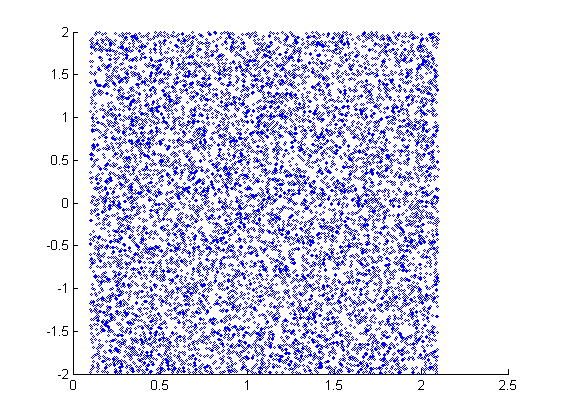
\includegraphics[width=\nn\textwidth]{Figs/col_m1_v1.png} 
& \hspace{-3mm} 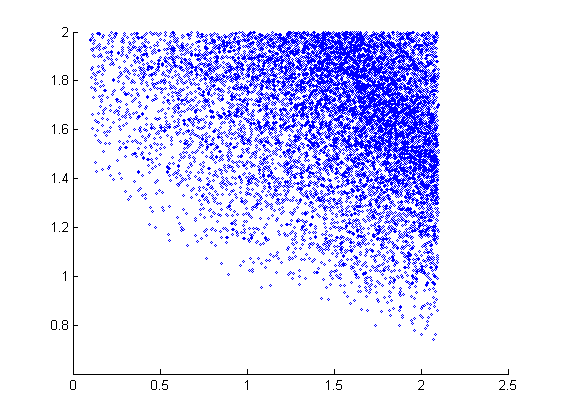
\includegraphics[width=\nn\textwidth]{Figs/col_m1v1_p3.png} 
& \hspace{-3mm} 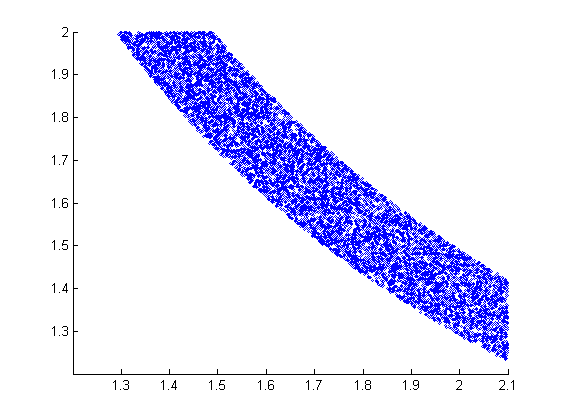
\includegraphics[width=\nn\textwidth]{Figs/col_m1v1_when_p_is_3_and_v2_is_0_dot_2.png}
& \hspace{-3mm} 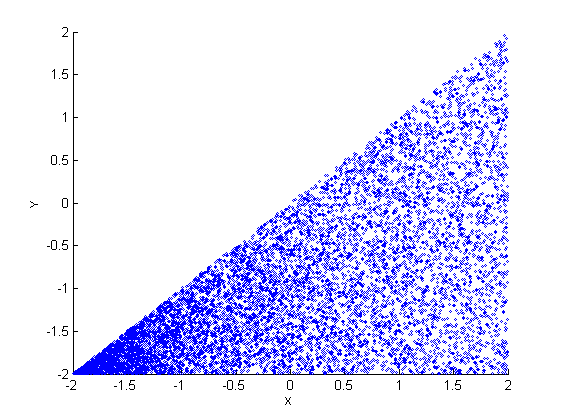
\includegraphics[width=\nn\textwidth]{Figs/col_v1v2.png}
& \hspace{-3mm} 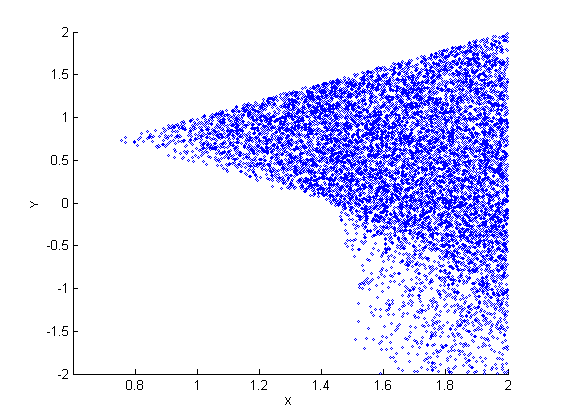
\includegraphics[width=\nn\textwidth]{Figs/col_v1v2whenPis3.png}
& \hspace{-3mm} 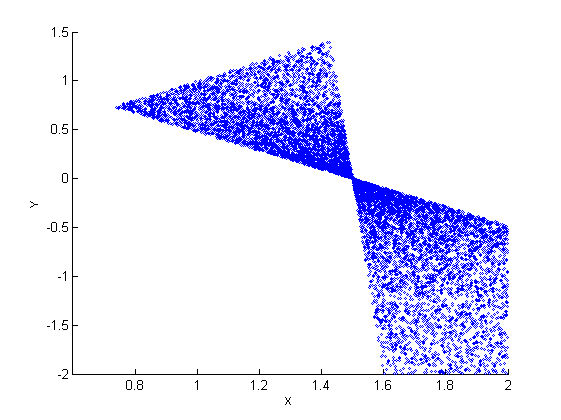
\includegraphics[width=\nn\textwidth]{Figs/colV1V2givenPis3M1is2.png}
\vspace{-1.5mm}
\\
   \hspace{-5mm} \footnotesize(a) 
& \hspace{-4mm} \footnotesize(b) 
& \hspace{-3mm} \footnotesize(c) 
&\hspace{-1mm} \footnotesize(d) 
&\hspace{-1mm} \footnotesize(e) 
&\hspace{-1mm} \footnotesize(f)\\
\multicolumn{6}{c}{}
\end{tabular}
\end{center}
\vspace{-8mm}
\caption{\footnotesize
Prior/posterior joint distributions of pairs of random variables in the \emph{collision} example. 
(a) $\pr(M_1, V_1)$,
(b) $\pr(M_1, V_1 \, | \, P_\text{tot} = 3)$,
(c) $\pr(M_1, V_1 \, | \, P_\text{tot} = 3, V_2 = 0.2)$,
(d) $\pr(V_1, V_2)$,
(e) $\pr(V_1, V_2 \, | \, P_\text{tot} = 3)$,
(f) $\pr(V_1, V_2 \, | \, M_1 =2, P_\text{tot} = 3)$
using rejection sampling on the $\delta$-collapsed model.
} 
\label{fig:mom}
\end{figure*}
%%%%%%%%%%%%%%%%%%%%%%%%%%%%%%%%%%%%%%%%%%%%%%%%%%%%%%%%%%%%%%%%%%%%%%%%%%


%FIG BLUE 2
%%%%%%%%%%%%%%%%%%%%%%%%%%%%%%%%%%%%%%%%%%%%%%%%%%%%%%%%%%%%%%%%%%%%%%%%%%
\begin{figure*}[t!]
\vspace{-1mm}
\begin{center}
\begin{tabular}{cccccc}
\hspace{-3mm}
{\footnotesize SymGibbs} 
&
{\footnotesize MH}
&
{\footnotesize HMC (high noise)}
&
{\footnotesize HMC (low noise)}
&
{\footnotesize SMC (high noise)}
&
{\footnotesize SMC (low noise)}
\\
   \hspace{-5mm} 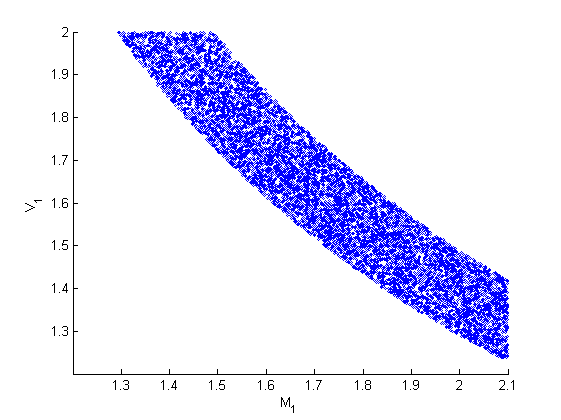
\includegraphics[width=\nn\textwidth]{Figs2/col_c_gibbs10000.png} 
& \hspace{-3mm} 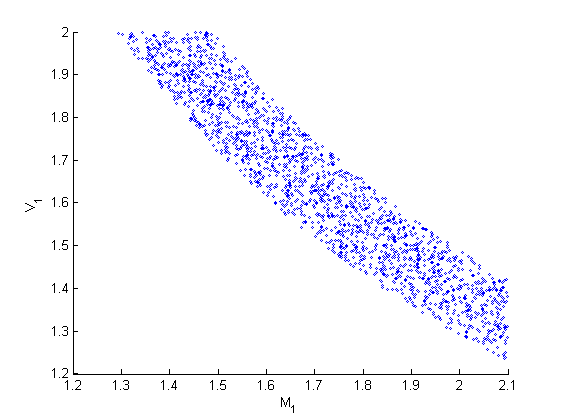
\includegraphics[width=\nn\textwidth]{Figs2/col-c-mh-10000_08.png} 
& \hspace{-3mm} 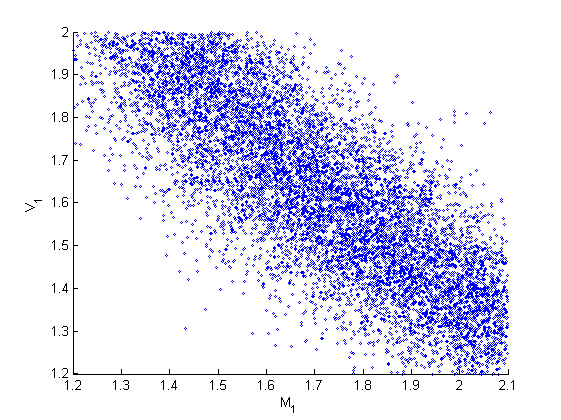
\includegraphics[width=\nn\textwidth]{Figs2/col_c_stan10000_02.png}
& \hspace{-3mm} 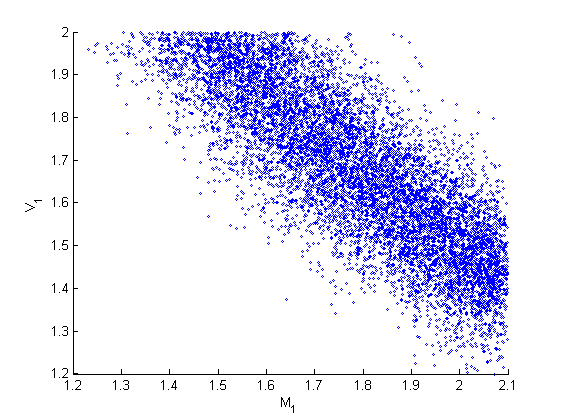
\includegraphics[width=\nn\textwidth]{Figs2/col_c_stan_10000_000001.png}
& \hspace{-3mm} 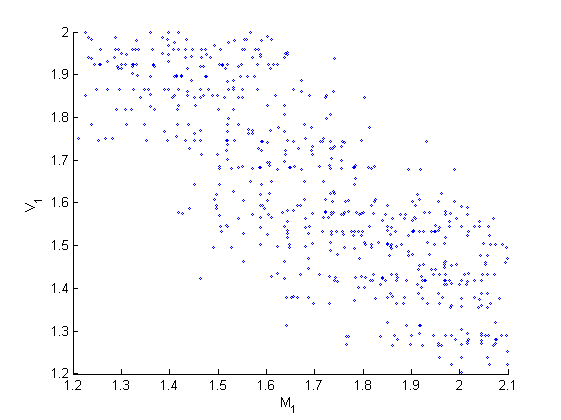
\includegraphics[width=\nn\textwidth]{Figs2/col_c_ang10000_02_001.png}
& \hspace{-3mm} 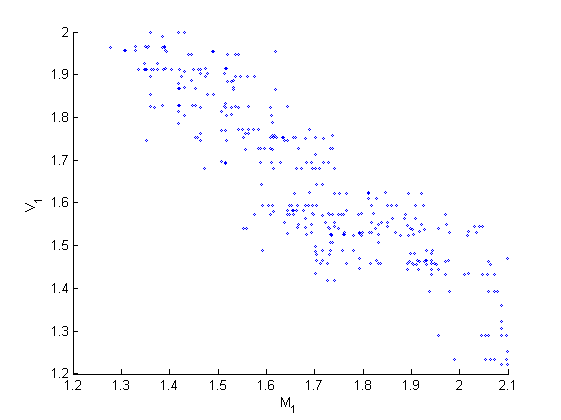
\includegraphics[width=\nn\textwidth]{Figs2/col_c_ang_10000_01_001}
\vspace{-1.5mm}
\\
   \hspace{-4mm} \footnotesize(a) 
& \hspace{-2mm} \footnotesize(b) 
& \hspace{-3mm} \footnotesize(c) 
&\hspace{-1mm} \footnotesize(d) 
&\hspace{-1mm} \footnotesize(e) 
&\hspace{-1mm} \footnotesize(f)\\
\multicolumn{6}{c}{}
\end{tabular}
\end{center}
\vspace{-8mm}
\caption{\footnotesize
10000 samples taken from the distribution Fig.~(\ref{fig:mom}-c)
using (a) Symbolic Gibbs sampler and(b) MH with \emph{proposal variance} 0.8 
on the reduced-dimension model as well as  
(c) Hamiltonian Monte Carlo (HMC) with a measurement error variance 0.2, 
, (d) and 0.01 as well as Anglican implementation of SMC alg. with %RDB alg. with 
parameters (e)
%$V_2$ and $P_\text{tot}$ observation noise variance 
$\sigma^2_{V_2} = 0.01$, $\sigma^2_{P_\text{tot}} = 0.2$ and 
(f) $\sigma^2_{V_2} = 0.01$, $\sigma^2_{P_\text{tot}} = 0.1$
on the \emph{approximated-by-noise} model.
}
\label{fig:mom2}
\vspace{-4mm}
\end{figure*}
%%%%%%%%%%%%%%%%%%%%%%%%%%%%%%%%%%%%%%%%%%%%%%%%%%%%%%%%%%%%%%%%%%%%%%%%%%

%%%%%%%%%%%%%%%%%%%%%%%%%%%%%%%%%%%%%%%%%%%%%%%%%%%%%%%%
\section{Experimental Results}
\label{sect:experimental.results}

Our experiments are to study the 
following questions:
\vspace{-2mm}
\begin{enumerate}[label=(\alph*)]
\item {\bf Posterior quality.} What are the qualities of the posteriors generated by conditioning on determinism in terms of their modality, continuity, shape of support, etc.?
\item {\bf MCMC comparison.} How is the performance of Symbolic Gibbs vs.\ other MCMC methods on such posteriors
(in terms of the convergence rate to the ground truth)?
\item {\bf Handling determinism.} How is the sampling performance affected if instead of $\delta$-collapsing,  the deterministic constraints are relaxed by noise (as done in previous work)? 
\end{enumerate}
\vspace{-2mm}
The compared MCMC algorithms, 
the utilized measurements
and the experimental models  
are introduced in 
Sections~\ref{sect:experimental.results.algorithms},
\ref{sect:experimental.results.measures} 
and \ref{sect:experimental.results.models}
respectively.
The experiments evaluations are discussed in in 
Section~\ref{sect:experimental.evaluations}.

%In the following subsection, we introduce the algorithms that are to be compared with out proposed algorithm using the measurements presented in Section~\ref{sect:experimental.results.measures} on three models presented and discussed in Section~\ref{sect:experimental.results.models}. 


\subsection{Algorithms} 
\label{sect:experimental.results.algorithms}
We compare the proposed \emph{symbolic Gibbs sampler} (SymGibbs) to
\emph{baseline Gibbs} (BaseGibbs) \citep{pearl1987evidential},
%i.e.\ where CDF is computed per sample, 
\emph{rejection sampling} (Rej) \citep{hammersley1964monte}, 
\emph{tuned Metropolis-Hastings} (MH) \citep{roberts1997weak}, 
\emph{Hamiltonian Monte Carlo} (HMC) using Stan PPL \citep{stan-manual:2014}
and \emph{Sequential Monte Carlo} (SMC) using Anglican PPL \citep{wood2014new}.\footnote{
We also tested the other algorithm implemented by Anglican, namely 
\emph{Particle-Gibbs} (PGibbs) (a variation of Particle-MCMC\citep{andrieu2010particle}) \
and \emph{random database} (RDB) (an MH-based algorithm introduced in \citep{wingate2011lightweight}) (see \cite{wood2014new}).
In our experimental models, the performance of these algorithms is very similar to (SMC).
Therefore, for the readability of the plots, we did not depict them.
}

SymGibbs, BaseGibbs and MH are run on \emph{$\delta$-collapsed} models while in the case of HMC and SMC, determinism is softened by observation noise. %(as required by Stan and Anglican PPLs).
Note that adding noise to the observation is the simplest and most commonly used method of dealing with determinism\citep{patil2010pymc}.\footnote{
For example in the collision model, the observation $P_{\text{tot}} = 3$  would be 
approximated with a normal distribution
{\footnotesize $\mathcal{N}( M_1 V_1 + M_2 V_2 - 3, \sigma_\eta^2)$}  
where the variance $\sigma_\eta^2$ is the noise parameter.
}

SymGibbs and BaseGibbs require no tunings. 
MH is automatically tuned after \citep{roberts1997weak} by testing 200 equidistant proposal variances in interval 
$(0, 0.1]$ and accepting a variance for which the acceptance rate closer to 0.24.

To soften the determinism in HMC and SMC,
the observation of a deterministic variable $Z$ %with prior $\delta\big( G_j(\cdot) - Z_j \big)$ 
is approximated by observation of a newly introduced variable 
with a Gaussian prior centered at $Z$ and with noise variance (parameter) $\sigma^2_{Z}$. 
%instead of conditioning on a deterministic variable $X$, it is assumed that a newly introduced stochastic variable $X'$ is observed whose prior is a Gaussian centered at $X$ and with noise variance (parameter) $\sigma^2_{X}$.
Anglican's syntax requires %promotes 
adding noise to all observed variables. Therefore, in the case of SMC, stochastic observations are also associated with noise parameters.
All used parameters are summarized in Table~\ref{t:parameters}. 
SymGibbs, BaseGibbs, Rej and MH have single thread java implementations.
The number of threads and other unspecified parameters of Stan and Anglican are their default settings.   
All algorithms run on a 4 core, 3.40GHz PC.% and the model compilation time of Stan and Anglican is not taken into account. 

\subsection{Measurements}
\label{sect:experimental.results.measures}
In each experiment, all non-observed stochastic random variables of the model  form the query vector $\bvec{Q} = [Q_1, \ldots, Q_\zeta]$.
The number of samples taken by a Markov chain $\Gamma$ up to a time $t$ is denoted by $n_{\Gamma}^t$ and  
the samples are denoted by 
$\bvec{q}_\Gamma^{(1)}, \ldots, \bvec{q}^{(n_{\Gamma}^t)}_\Gamma$
where $\bvec{q}_\Gamma^{(i)} := 
[q_{1, \Gamma}^{(i)} , \ldots, q_{\zeta, \Gamma}^{(i)}]$

{\bf 1. Mean absolute error vs time.}
The main measurement 
is to compute the \emph{mean absolute error} (MAE) 
\begin{equation}\footnotesize
\label{e:error.vs.time.measure}
\textsc{MAE}_{\Gamma}(t) := \frac{1}{\zeta \cdot n_\Gamma^t} 
\sum_{j=1}^{\zeta}
\sum_{i=1}^{n_\Gamma^t}
\left|{q}^{(i)}_{j, \Gamma} - {q}_j^* \right|
\end{equation}
vs (wall-clock) time $t$ where 
$\bvec{q}^* := [q_1^*, \ldots q_\zeta^*]$ 
is the ground truth mean query vector (that will be discussed shortly).

In each experiment and for each algorithm, $\gamma = 15$ Markov chains are run,  and for each time point $t$,
average and standard error of %mean absolute errors 
$\textsc{MAE}_{1}(t)$ to $\textsc{MAE}_{\gamma}(t)$
are plotted. 

{\bf 2. Time to reach error threshold ($\boldsymbol\tau$).}
%In experiments where the model size is variable,
%We illustrate MAE vs time for a couple of size configurations.
%the space restrictions does not allow us to illustrate 
This is a single plot that summarizes the overall behavior of each sampler algorithm w.r.t.\ the model size:
We notice that after some error threshold, the comparative performance of the samplers remains fixed.
Therefore, for each sampler, the time to reach a fixed threshold $\tau$ is plotted vs the model size.

If we pick the error threshold too low, many samplers will never reach it. 
If it is too high, samplers pass it prior to be comparatively stable. 
Per experiment, we manually choose  an error threshold that provides a fair compromise between these two requirements
(see Table~\ref{t:parameters}).

\subsubsection*{Ground truth (of mean query vector) $(\bvec{q}^*)$}
In the first experimental model (asymmetric collision model)
the ground truth is approximated by taking 200,000 samples via \emph{rejection sampling} (Rej)
(as a completely unbiased sampler).
However, this approximation cannot be used in high-dimensional models
since the the performance of Rej drastically deteriorates with increasing dimension.
%In low dimensional models 
%the ground truth (required in Eq.~(\ref{e:error.vs.time.measure}))
%is approximated by taking sufficiently large number of samples by rejection sampling (as a completely unbiased sampler).
%However, in the experiments where the model size is parametric, we cannot rely on rejection sampling since its performance on the studied model deteriorates drastically in dimension. 
%We cannot rely on \emph{MCMC convergence diagnostics} methods \citep{cowles1996markov} because they can produce misleading results in case Markov chains do not converge to the ground truth; a scenario that as we will see, for highly complex posteriors is not improbable.
Our remaining experimental models are intentionally chosen to be symmetric
as this enables us to compute the ground truth manually.% rather than relying on Rej.
%Our solution is to conduct tests on symmetric models for which the posterior ground truth can be computed manually.


\subsection{Experimental models}
\label{sect:experimental.results.models}

%Our experiments are to study
%(a) the quality of the posterior joints, 
%(b) the error and convergence rate of MCMC methods and %the mixing rate of MCMC methods and
%(c) the effect of approximation of hard constraints in models with deterministic conditionals. 

%The three experimental models are as follows:
%\subsubsection{(Asymmetric) collision model.}\label{sect:model1} 
{\bf(Asymmetric) collision model.}  
The first model is our running example introduced in 
Section~\ref{sect:intro} (the \emph{collision model}) using which: 
\vspace{-2mm}
\begin{enumerate}
\item To study the posterior quality, for different evidence and queries, joint posteriors are approximated by 10000 samples taken via rejection sampling
and plotted in Figure~\ref{fig:mom}.
\item    
To  compare sampling methods (qualitatively), 
in Figure~\ref{fig:mom2}, the experiment is repeated on the posterior of 
Figure~\ref{fig:mom}-c using the sampling algorithms described in Section~\ref{sect:experimental.results.algorithms}
\item
For qualitative MCMC comparison, \emph{absolute error vs time}
is plotted in Figure~\ref{fig:asymmetric}).
\end{enumerate}

With increasing the number of space variables, the performance of different sampling algorithms significantly varies.
Therefore,
in the remaining experiments, comparisons take place w.r.t.\ the variable space dimensionality.
 
%Fig todo
%%%%%%%%%%%%%%%%%%%%%%%%%%%%%%%%%%%%%%%%%%%%%%%%%%%%%%%%
\begin{figure}
\centering
     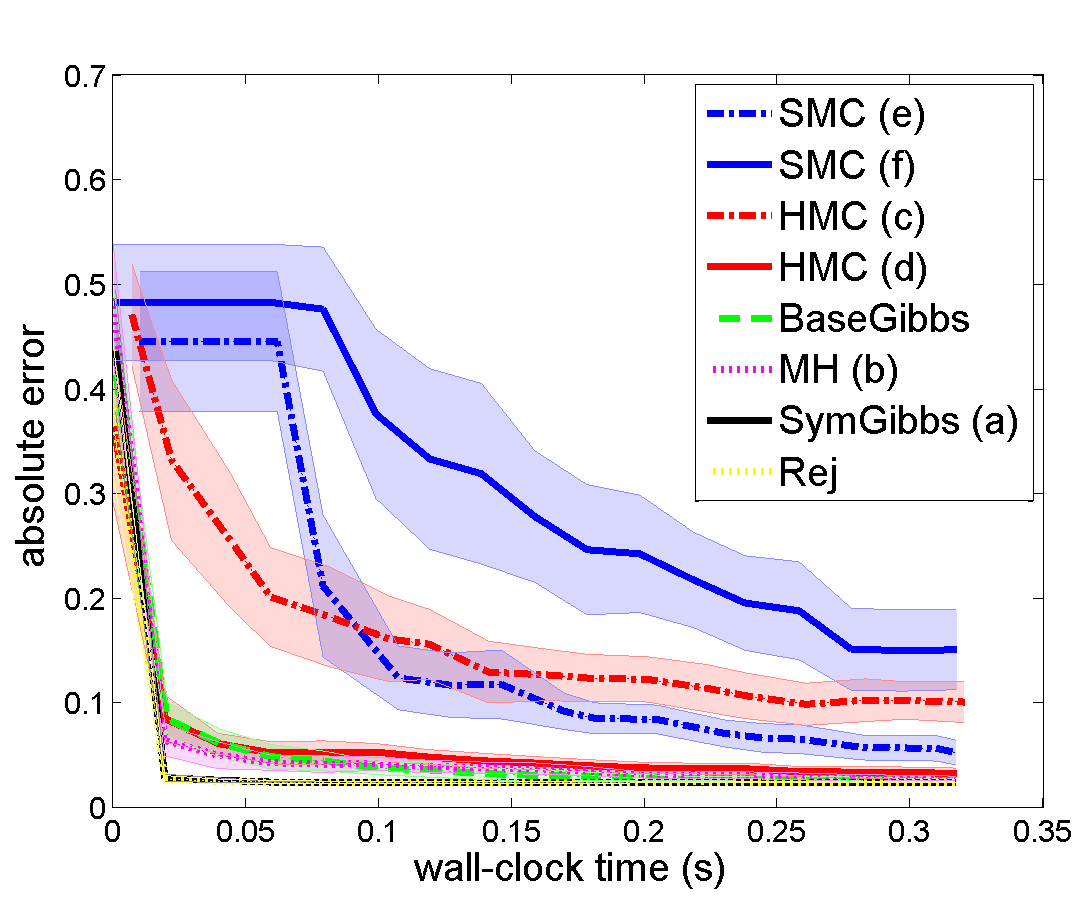
\includegraphics[width=0.8\linewidth, height=125pt]
{plotsx/vis-col/err-vs-time__param2-shaded.pdf}
%{Figs/plots/collision/err-vs-time__param4-shaded.pdf}
      \caption{
%Error as a function of wall clock time (s) for the (asymmetric) collision model using MCMCs with same configurations as in Figure~\ref{fig:mom2}. 
Absolute error vs time in the \emph{asymmetric collision model}. (The algorithms correspond sub-figures of Fig.~\ref{fig:mom2}.)
 }
\label{fig:asymmetric}
\end{figure}





%Ex 2;  Fig 1
%%%%%%%%%%%%%%%%%%%%%%%%%%%%%%%%%%%%%%%%%%%%%%%%%%%%%%%%%%%%%%%%%%%%%%%%%%
\begin{figure*}[t!]
\vspace{-0mm}
\begin{center}
\begin{tabular}{ccc}
   \hspace{-5mm} 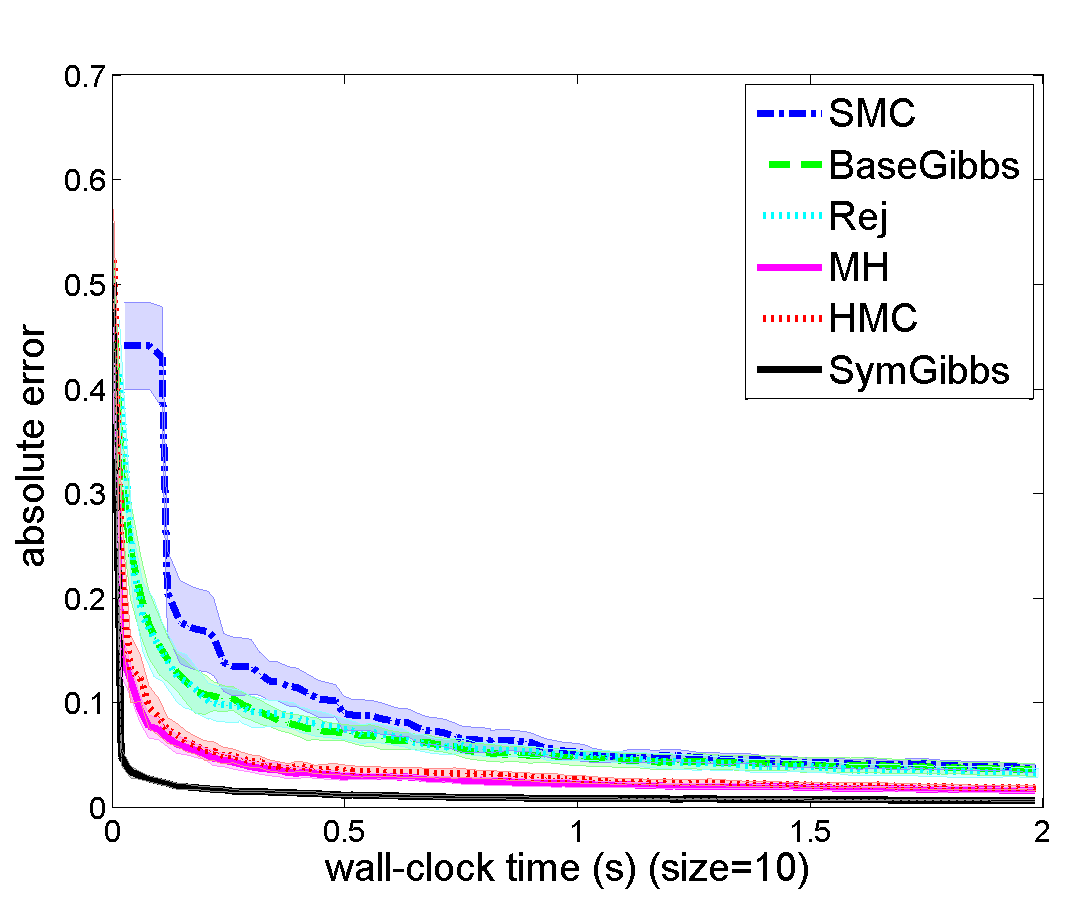
\includegraphics[width=\nnn\textwidth, height=\nnh\textwidth]{plotsx/collisionx/err-vs-time__param5-shaded.pdf} 
& \hspace{-3mm} 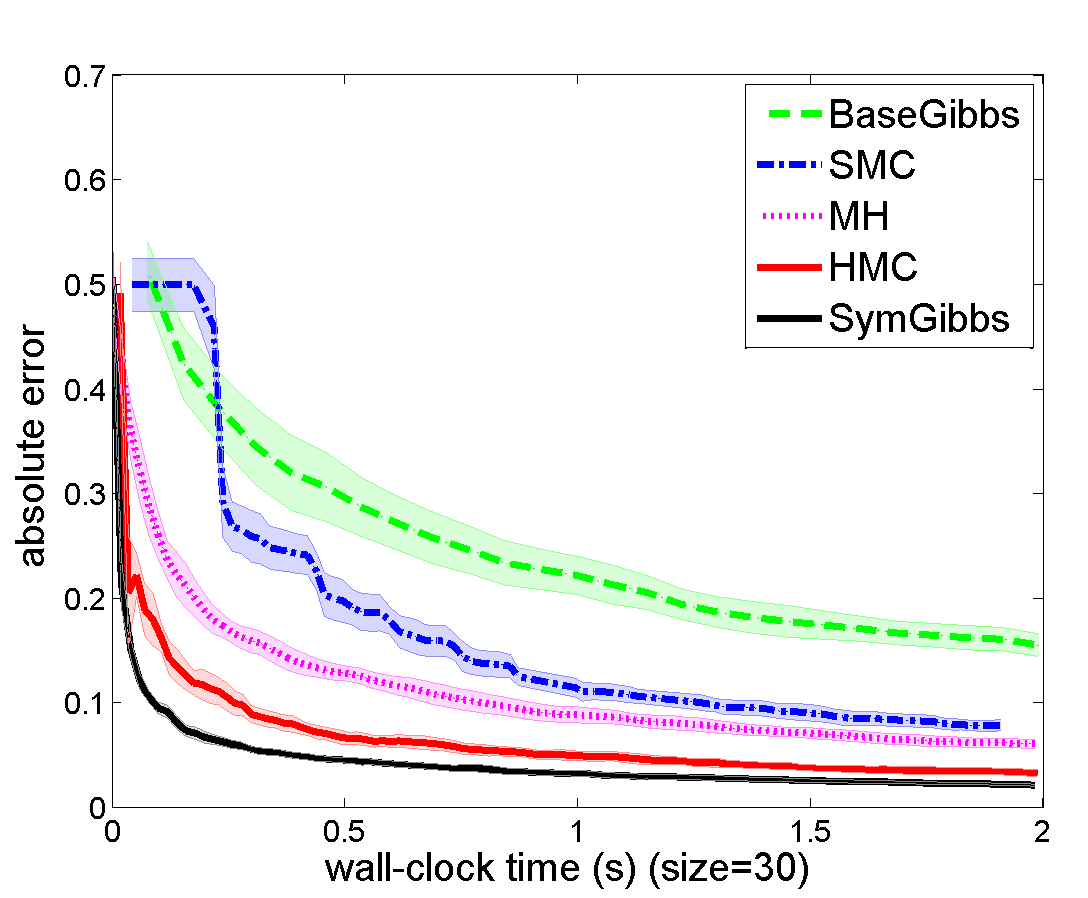
\includegraphics[width=\nnn\textwidth, height=\nnh\textwidth]{plotsx/collisionx/err-vs-time__param15-shaded.pdf} 
& \hspace{-3mm} 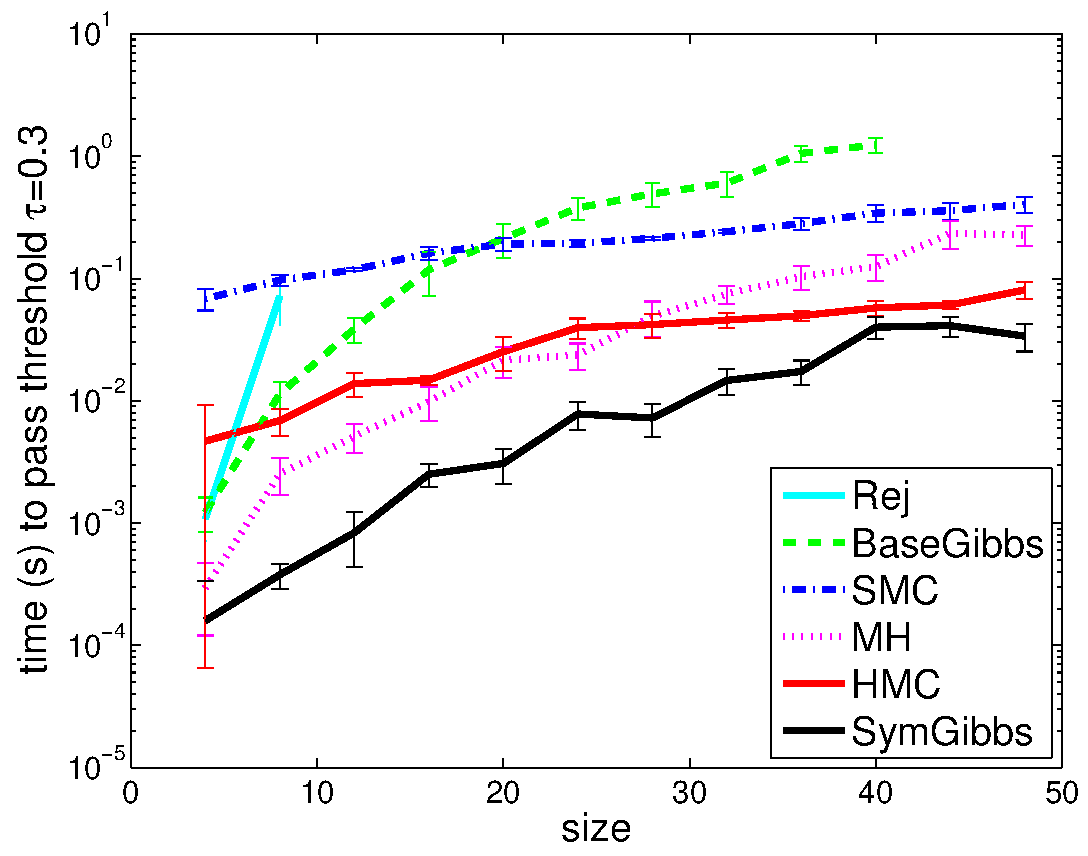
\includegraphics[width=\nnn\textwidth, height=\nnh\textwidth]{plotsx/collisionx/time_vs_param-errorbar.pdf}%collision/collisionTimeVsSize.png}
\vspace{-1.5mm}
\\
\hspace{-5mm} \footnotesize(a) 
& \hspace{-4mm} \footnotesize(b) 
& \hspace{-3mm} \footnotesize(c) \\
\multicolumn{3}{c}{}
\end{tabular}
\end{center}
\vspace{-8mm}
\caption{\footnotesize 
MCMC Convergence measurements in the symmetric multi-object collision model: 
Absolute error vs time for collision of (a) 4 and (b) 20 objects; (c) Time to reach error threshold $\tau=0.3$.}
\label{fig:multi-object.mom}
\vspace{-4mm}
\end{figure*}
%%%%%%%%%%%%%%%%%%%%%%%%%%%%%%%%%%%%%%%%%%%%%%%%%%%%%%%%%%%%%%%%%%%%%%%%%%


%Ex 2;  Fig 1
%%%%%%%%%%%%%%%%%%%%%%%%%%%%%%%%%%%%%%%%%%%%%%%%%%%%%%%%%%%%%%%%%%%%%%%%%%
\begin{figure*}[t!]
\vspace{-0mm}
\begin{center}
\begin{tabular}{ccc}
   \hspace{-5mm} 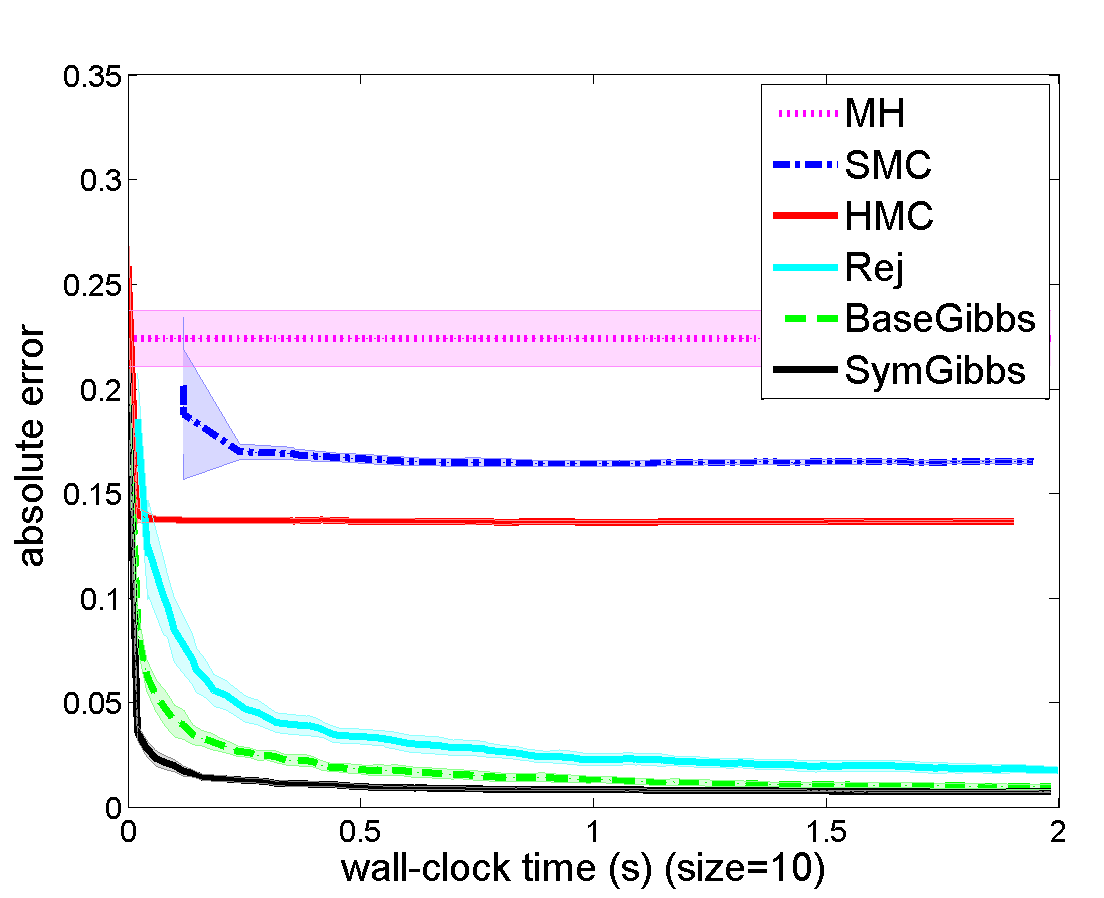
\includegraphics[width=\nnn\textwidth, height=\nnh\textwidth]{plotsx/conductancex/err-vs-time__param10-shaded.pdf} 
& \hspace{-3mm} 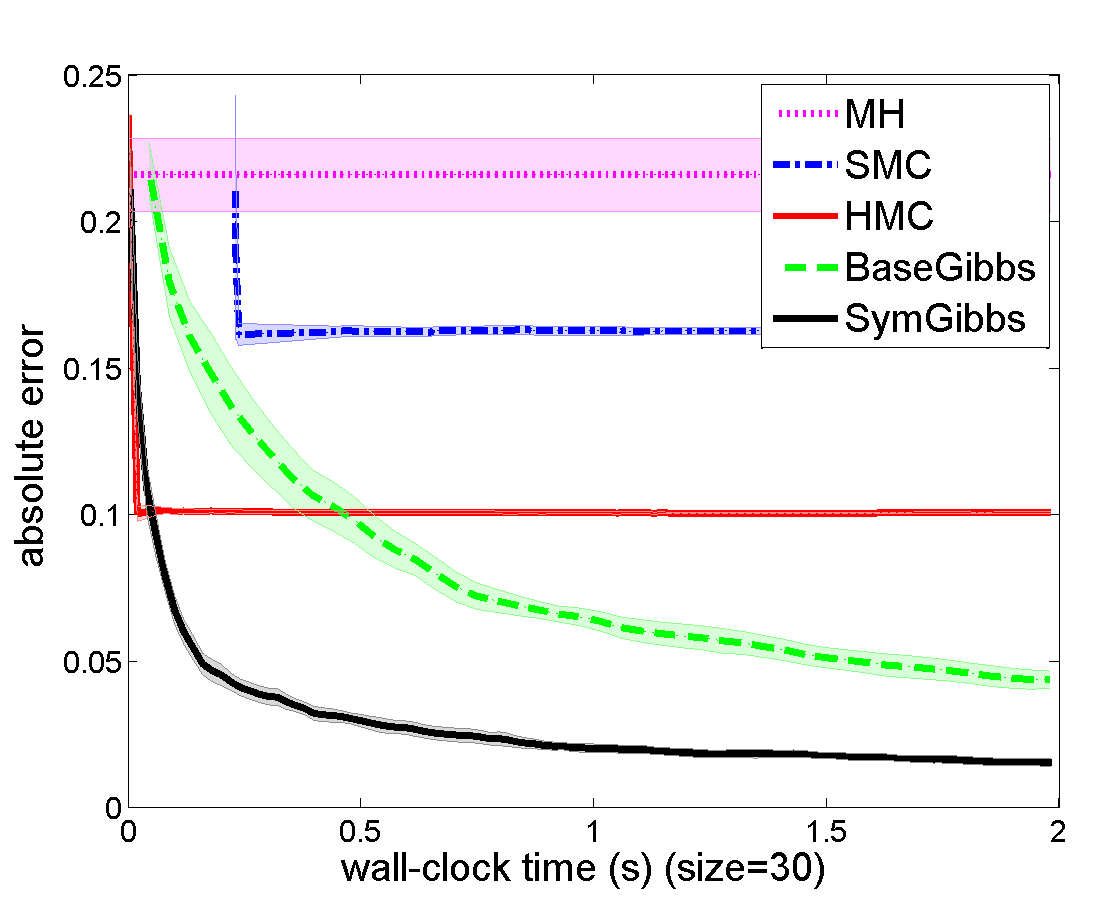
\includegraphics[width=\nnn\textwidth, height=\nnh\textwidth]{plotsx/conductancex/err-vs-time__param30-shaded.pdf} 
& \hspace{-3mm} 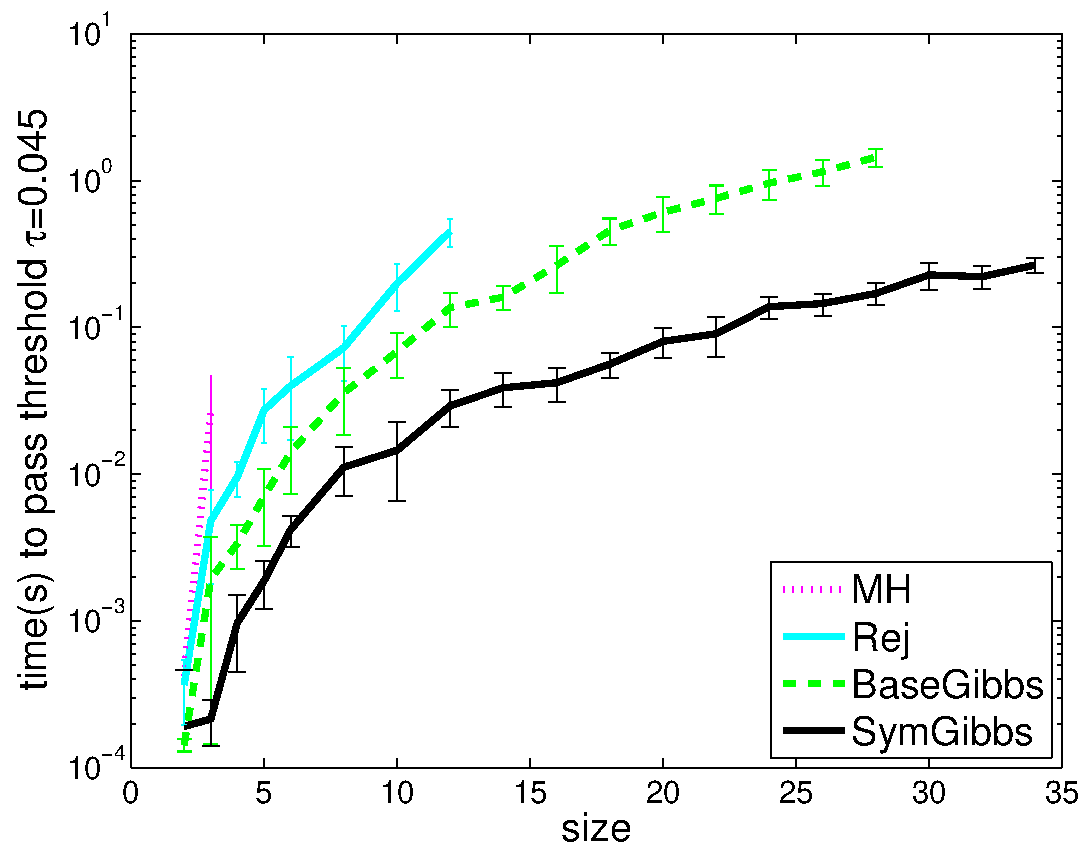
\includegraphics[width=\nnn\textwidth, height=\nnh\textwidth]{plotsx/conductancex/time_vs_param-errorbar.pdf}
\vspace{-1.5mm}
\\
\hspace{-5mm} \footnotesize(a) 
& \hspace{-4mm} \footnotesize(b) 
& \hspace{-3mm} \footnotesize(c) \\
\multicolumn{3}{c}{}
\end{tabular}
\end{center}
\vspace{-8mm}
\caption{\footnotesize 
MCMC Convergence measurements in the building wiring model: 
Absolute error vs time for a model with (a) size 4 (i.e.\ 4 paralleled resistors) and (b) size 30; (c) Time to reach error threshold $\tau=0.045$.}
\label{fig:resistor}
\vspace{-4mm}
\end{figure*}
%%%%%%%%%%%%%%%%%%%%%%%%%%%%%%%%%%%%%%%%%%%%%%%%%%%%%%%%%%%%%%%%%%%%%%%%%%




%\subsubsection{Symmetric multi-object collision model} %In the second experiment,
{\bf Symmetric multi-object collision model.} %In the second experiment,
%We study the role of model size on the performance of MCMC methods. We cannot rely on \emph{MCMC convergence diagnostics} methods \citep{cowles1996markov} because they can produce misleading results in case MCMCs do not converge to the ground truth, a scenario that as we will see, for highly complex posteriors is not improbable. Meanwhile, we cannot rely on rejection sampling to approximate the Ground truth since its performance on the studied model deteriorates drastically in dimension. Our solution is to conduct tests on symmetric models for which the posterior ground truth can be computed manually.
Consider a variation of the collision model in which $n$ objects collide.  
%by assuming that %collide. But we omit the sequential dependencies of velocities s.t.\ 
Let all $V_i$ and $M_i$ share a same uniform prior $U(0.2, 2.2)$ and the constraint be $\sum_{i=1}^n{M_i V_i} = P_{\text{tot}}$. 
The symmetry enables us to compute the posterior ground truth means  values  manually:
\begin{equation}\footnotesize
\label{e:col.GT}
M^* = V^* = \sqrt{P_{\text{tot}} / n} %\left(\frac{P}{n}\right)^{0.5}
\end{equation}
Conditioned on $P_{\text{tot}} = 1.5 n$, all masses $M_i$ and velocities  $V_i$ are queried. 
%The tested algorithms running on the reduced-dim posterior are: symbolic Gibbs (see Section~\ref{sect:symbolic.gibbs}), 
%baseline Gibbs (CDF computation per sample), 
%MH (Metropolis-Hastings tuned manually), 
%MH automatically tuned %to reach the acceptance rate of 0.234 
%after \citep{roberts1997weak})\footnote{\label{foot:tuning} Among 200 equidistant proposal variances in %interval $(0, 0.1]$ 
%the one is chosen for which the acceptance rate is closer to 0.24. } and rejection sampling. Among the samplers that add noise to determinism, Stan's Hamiltonian MCMC with noise (variance) parameter $\sigma_P = 0.05$ and Anglican's SMC with noise parameter $0.1$ are plotted. The noise parameters are chosen manually trying to maximize the convergence rate. Other parameters are Stan and Anglican's default setting.
%By (\ref{e:col.GT}), $a_k$, the average  of $k$-th sample vector $\bvec{s}^{(k)}$, is expected to be $\sqrt{1.5}$; therefore, as the overall sampling error measure, 
%$\mathbb{E}[|{\xi} - {\xi}^*|]$ 
%$\mathbb{E}[|\bvec{a} - \bvec{a}^*|]$ is computed where $\bvec{a}$ is the vector of $a_k$ (for $k$ ranges be the number of taken samples) and all entries of vector $\bvec{a}^*$ are 1.5.
By (\ref{e:col.GT}), all elements of the ground truth vector $\bvec{q}^*$ are $\sqrt{1.5}$.

%For each algorithm 15 Markov chains are run and at consecutive time slots, their corresponding point-to-point means and standard errors are computed. 
MAE vs. time is depicted in Figures~\ref{fig:multi-object.mom}.a \& b for a 10-D and a 30-D model, respectively.
%\footnote{Note that the dimensionality of the random variable space is twice the number of objects because each object is associated with a mass and a velocity node. %Conditioned on the total momentum, reduced-dim space is 19D and algorithms that add noise to the observation, deal with  a 21D space.} 
Time to reach error threshold $\tau = 0.3$ is plotted in 
Figure~\ref{fig:multi-object.mom}.c.

%We repeated the experiment for different model sizes but for the sake of space restrictions, we do not depict each plot individually. Instead we provide a single plot that summarizes the overall behavior of each sampler w.r.t.\ the model size. We notice that after a particular threshold, the comparative performance of the samplers remains fixed. Therefore, in Figure ???, for each sampler the (wall-clock) time (s) to reach a sampling error threshold (average) equal to 0.3 is plotted vs the model size.\footnote{ If we pick the error threshold to be too low, many samplers would never reach it. If it is too high, samplers pass it prior to be comparatively stable. On collision model, the manual error threshold choice (around) 0.3 happens to provide a fair compromise between these two requirements.  }%end footnote

  
%In the latter high-dimensional space, the rejection sampling has not been able to generate a particle. MH algorithms convergence rate is very low while the baseline Gibbs still perform well and the symbolic Gibbs performance is at least an order of magnitude better. Finally, Figure~\ref{fig:err-threshold-vs-size-collision} depicts the time to reach a fixed error threshold $T=0.2$ versus number of colliding objects. \\
%

The next model deals with a more complicated observed determinism.

{\bf Building wiring model. } 
An electrical circuit composed of $n$, $10\Omega\pm5\%$ parallel resistor elements $R_i$
(with priors $\pr(R_i) = U(9.5, \, 10.5)$).
% with bell-shaped tolerance distributions (truncated quadratics, positive in the range $[8, 12]$). The posterior tolerance distribution is computed when 
The resistors are inaccessible i.e.\ the voltage drop and the current associated with them cannot be measured directly.
Given the source voltage $V$ and the total input current $I$, the posterior distribution of the element resistances are required.
Here the deterministic constraint is:
%Here, the observation can be stated as the following deterministic constraint:
\begin{equation} \footnotesize 
\label{e:reduced.mass}
 \frac{1}{R_1} + \ldots + \frac{1}{R_n} = c
\end{equation}
where $c = \frac{I}{V}$.
Equations if the form (\ref{e:reduced.mass}) are generally referred to as \emph{reduced mass} relationships and 
have applications in the electrical, thermal, hydraulic and mechanical engineering domains.

Let the observation be $c = {3n}/{(2*10.5 + 9.5)}$.
Due to the symmetry of the problem, the posterior ground truth mean is known:
\begin{equation*}
R_i^* = \frac{n}{c} = 10.166667\qquad \text{ for } i = 1, \ldots, n
\end{equation*}
MAE vs. time for networks of 10 and 30 resistors are depicted in 
Figures~\ref{fig:resistor}.a \& b respectively.
Time to reach error threshold $\tau = 0.045$ is plotted in 
Figure~\ref{fig:resistor}.c.

%Stan and Anglican observation noise divergences are 0.02 and 0.07 respectively. Other settings are as before.

\subsection{Experimental evaluations}
\label{sect:experimental.evaluations}
Given the experimental results, 
the questions posed in the beginning of this section are replied as follows:

{\bf Posterior quality.} 
Plots of Figure~\ref{fig:mom} illustrate the posterior quality of the models studied in this paper.
They show that  
even in the presence of a single deterministic constraint, 
a simple prior can be transformed into a complicated piecewise and multi-modal posterior that does not resemble any family of 
probability densities studied in the literature so far. 

{\bf MCMC comparison}
Plots of Figure~\ref{fig:mom2} shows that MH and SMC suffer from low \emph{effective sample size}. 
Note that the apparent sparsity of plots~\ref{fig:mom2}-b, \ref{fig:mom2}-e \& \ref{fig:mom2}-f is due to repeated samples (rejected proposals).

The carried out quantitative measurements 
(Figures~\ref{fig:asymmetric},  \ref{fig:multi-object.mom} and \ref{fig:resistor}) 
indicate that in all experimental settings,
Symbolic Gibbs constantly and significantly performs the best.



{\bf Handling determinism}
%Plots Fig.~\ref{fig:mom2}-c and Fig.~\ref{fig:mom2}-d suggest  that  softening determinism by noise leads to a  discrepancy between the model and taken samples that may not be resolved by lowering the noise threshold (i.e.\ decreasing HMC's observation noise variance from 0.2 to 0.001 (Fig.~\ref{fig:mom2}-d) does not help much.
All quantitative measurements 
(Figures~\ref{fig:asymmetric},  \ref{fig:multi-object.mom} and 
\ref{fig:resistor})
indicate that approximating the determinism by noise leads to poor results.
It should be mentioned that 
the state-of-the-art probabilistic programming languages (PPLs),
disallow deterministic relationships among continuous random variables 
be observed.\footnote{
In BUGS \citep{lunn2009bugs}, the popular software for analysis of statistical models, \emph{logical nodes} cannot be given data or initial values .
In PyMC \citep{patil2010pymc} deterministic variables have no \emph{observed flag}. 
In Stan \citep{stan-manual:2014} 
if you try to assign an observation value to a deterministic variable, you will encounter an error message: 
``attempt to assign variable in wrong block'' while 
Anglican \citep{wood2014new} throws error ``invalid-observe", etc.}
The solution that these off-the-shelf inference frameworks suggest (or impose) is to approximate the observed determinism via adding noise to the observation 
\citep{wood2014new}.
%(hard to soft constraint conversion via introducing measurement error)


% ................................................................................................ 



An interesting result is that in the Building wiring model, even in a dimensionality as low as 10, 
the Metropolis-Hasting based algorithms (i.e.\ HM, HMC and SMC) may not converge to the (manually computed) ground truth or their convergence rate is extremely low. 
This happens regardless of the way determinism is handled. 
A reason may be as follows:
It is widely known that all Metropolis-Hasting-based algorithms are sensitive to parameter tunings.
Tuning takes place internally and during the burn-in period according to some heuristics.
Such heuristics may not be valid in the densities studied in this paper as they are very different from the bell-shaped unimodal distributions often studied in the literature so far.

%Manual computations verified that in the Building wiring model, high degree terms occur in the denominator of the posterior fraction. This may be another reason for the poor performance of the Metropolis-Hasting-based algorithms: Existence of multiple highly dense regions in the posterior can act as traps for such algorithms.

Since Gibbs samplers directly sample from the original distributions (rather than proposal densities) they can cope well with anomalies and as our results show, always converge to the ground truth. 

%Here and in the quantitative experiments that will follow, regardless to the parameter tuning, the performance of algorithms where determinism is softened by noise is much lower than the algorithms with $\delta$-collapsed models.

 \section{Conclusion}
\label{sect:conclusion}
Recently, piecewise polynomial distributions have attracted attention.
So far, piecewise polynomials with hyperrectangular, hyper-rhombus and linear partitioning constraints have been used in Bayesian networks \citep{shenoy2011inference,shenoy2012two,Sanner:12}.

In this paper we introduced polynomial piecewise fractional functions (PPFs).
They are are polynomial fractions with polynomial partitioning constraints
and up to our knowledge, are the richest class of piecewise functions studied in the literature of graphical models and probabilistic inference so far.
We showed that this family is expressive enough to remain closed under operations required to 
transform networks with (non)linear deterministic restrictions, to purely stochastic models.

We also showed that a large subset of PPFs have symbolic univariate integrals.
This led to the main contribution of this paper. 
A full automated exact Gibbs sampler, called \emph{symbolic Gibbs}, 
in which all univariate CDFs required for Gibbs sampling are computed analytically and prior to the actual sampling process.
Our novel sampling method, \emph{symbolic Gibbs}, saves a significant amount of computation, and improving the performance dramatically. The combination of these novel contributions should make probabilistic reasoning applicable to variety of new applications that have remained unsolvable so far. 

  


%*********************************************************************************************
%*********************************************************************************************
%*********************************************************************************************

% Note use of \abovespace and \belowspace to get reasonable spacing 
% above and below tabular lines. 

%\begin{table}[t]
%\caption{Classification accuracies for naive Bayes and flexible 
%Bayes on various data sets.}
%\label{sample-table}
%\vskip 0.15in
%\begin{center}
%\begin{small}
%\begin{sc}
%\begin{tabular}{lcccr}
%\hline
%\abovespace\belowspace
%Data set & Naive & Flexible & Better? \\
%\hline
%\abovespace
%Breast    & 95.9$\pm$ 0.2& 96.7$\pm$ 0.2& $\surd$ \\
%Cleveland & 83.3$\pm$ 0.6& 80.0$\pm$ 0.6& $\times$\\
%Glass2    & 61.9$\pm$ 1.4& 83.8$\pm$ 0.7& $\surd$ \\
%Credit    & 74.8$\pm$ 0.5& 78.3$\pm$ 0.6&         \\
%Horse     & 73.3$\pm$ 0.9& 69.7$\pm$ 1.0& $\times$\\
%Meta      & 67.1$\pm$ 0.6& 76.5$\pm$ 0.5& $\surd$ \\
%Pima      & 75.1$\pm$ 0.6& 73.9$\pm$ 0.5&         \\
%\belowspace
%Vehicle   & 44.9$\pm$ 0.6& 61.5$\pm$ 0.4& $\surd$ \\
%\hline
%\end{tabular}
%\end{sc}
%\end{small}
%\end{center}
%\vskip -0.1in
%\end{table}

%\subsubsection*{References}
{%\footnotesize
\bibliographystyle{plainnat}
\bibliography{symGibbsUAI}
%\bibliographystyle{icml2015}
}


\end{document}

======================================================

{\color{green}As mentioned, conditioning on deterministic constraints lead to posterior masses positioned  on submanifolds and transformations that are required for dimension reduction often end in distributions which are highly piecewise and multimodal. This class of distributions is intrinsically different from the smooth, bell-shaped distributions often studied in the literature. }

%We tested the algorithms supported by Anglican:  sequential Monte Carlo (SMC) \cite{wood2014new}, Particle-Gibbs (PGibbs) (a variation of Particle-MCMC\cite{andrieu2010particle})  and a variation of MH introduced in \cite{wingate2011lightweight} and named \emph{random database} (RDB) in \cite{wood2014new}. Due to existence of multiple noisy observations, in terms of size and accuracy of the effective samples, the performance of all three algorithms were low. The best performance was due to RDB which is plotted. 
 

\subsection{Monte Carlo methods.}
%An alternative to exact inference is to approximate the joint distribution by a set of samples drawn from it using Monte Carlo methods. By the law of large numbers, this approximation is asymptotically unbiased. Using samples, the costly marginalization operation is avoided since the conditional probability $\pr(\bvec{q} \,| \, \bvec{e})$ is simply approximated by the number of samples satisfying $\bvec{q} \cap \bvec{e}$ divided by the number of samples satisfying $\bvec{e}$.
%Note that unlike other approximate methods, inference via sampling leads to asymptotically unbiased solutions i.e.\ by taking sufficient number of samples, the \emph{posterior} can be approximated by an arbitrary precision.
Approximating the posterior distribution via drawing samples from it by Monte Carlo methods 
provides an asymptotically unbiased tool that completely avoids the hassle of multiple integrations.% required in closed-form sampling.   
Three major such methods are as follows:

{\bf Rejection sampling:} 
In this method \citep{hammersley1964monte}, to draw a sample from 
a distribution $p(\bvec{X})$, a sample $\bvec{x}$ is taken from another distribution $q(\bvec{X})$
such that $p(\bvec{X})/q(\bvec{X})$ is bound by a known constant $c$
and samples can be taken from $q(\bvec{X})$ efficiently.
The produced sample is accepted with probability $p(\bvec{x}) / c q(\bvec{x})$, 
otherwise it is rejected and the process is repeated. 

{\bf Metropolis-Hastings (MH):}
To draw a new sample $\bvec{x}^{(t)}$ from a distribution $p(\bvec{X})$, given a previously taken sample $\bvec{x}^{(t-1)}$, 
MH \citep{metropolis1953equation} takes a sample $\bvec{x}'$ from a symmetric \emph{proposal density} $q(\bvec{X} |\, \bvec{x}^{(t-1)})$. 
%from which samples can be taken efficiently 
%(often an isotropic \emph{Gaussian} centered at $\bvec{x}^{(t-1)}$). 
With probability $\min \big(1, p(\bvec{x}')/p(\bvec{x}^{(t-1)}) \big)$, 
$\bvec{x}'$ is accepted as the next sample ($\bvec{x}^{(t)} \leftarrow \bvec{x}'$), otherwise, $\bvec{x}^{(t)} \leftarrow \bvec{x}^{(t-1)}$. 
Choosing a good \emph{proposal} is problem-dependent and requires tuning. 


{\bf Gibbs sampling:}
Gibbs  \citep{geman1984stochastic} is a robust sampling tool in the sense that it does not require known bounds, tuned proposal densities or parameters.
Drawing a sample for $\bvec{X} = (X_1, \ldots, X_N)$ takes place in $N$ steps.
In the $i$-th step, $X_i$ is sampled conditioned on the last realization of the others:
$x_i \sim \pr(X_i \,|\, \bvec{x}_{-i})$. 
To perform this task, the following univariate \emph{Cumulative Distribution Function} (CDF)
is computed by equation~(\ref{e:cdf}) and samples are taken by inverse transform sampling. 
{\footnotesize
\begin{equation}
%\label{e:cdf}
F(X_i  \,|\, \bvec{x}_{-i}) 
\propto
\int_{-\infty}^{X_i} \!\!\!\! \pr(X_i = t, \bvec{x}_{-i}) \, d  t
\end{equation} 



\begin{algorithm}[tb]%[hb!]
\caption{{\sc $\delta$-Collapsing}  
\label{alg:posterior-joint}}
\begin{algorithmic}
\STATE {\bf Input: }{\small
$\tuple{\bvec{E}, \bvec{e}}$ 
// \emph{\small evidence (variables \bvec{E} and values \bvec{e})}\\
%$\bvec{Z} = \{Z\}$, deterministic variables\\
\hspace{11mm} 
$\small \boldsymbol{\Psi}$ % := \boldsymbol{\Psi^S} \cup \boldsymbol{\Psi^D}$ 
// \emph{\small union of stochastic potentials (in the form $\Psi_i$) and deterministic potentials (in the form $\delta\big( G_j (\cdot) - Z_j \big)$.}
 }
\STATE {\bf Output} {posterior joint distribution of a subset of variables from which, all other variables can be decided.}
 \vspace{2mm}
\hrule
 \vspace{2mm}
%----
\STATE{\bf 1.~Observed variable instantiation.} 
In all potentials (either deterministic or statistical), all observed stochastic/deterministic 
variables are instantiated: \vspace{-1.0mm}
%\footnote{ A deterministic factor $\delta[Z_j- G_j(\cdot)]$ associated with an observed variable $Z_j = c$ is therefore substituted by $\delta[c- G_j(\cdot)]$.}
\begin{equation*}\footnotesize 
\forall \Psi \in \boldsymbol{\Psi} \qquad \Psi \leftarrow \Psi|_{\bvec{E} \leftarrow \bvec{e}}
\end{equation*} 
%----
\STATE{\bf 2. Marginalizing determinism.} 
In all potentials, all deterministic variables $Z_j$, are 
substituted by their 
logical values $G_j(\cdot)$ (so, the potential $\delta ( G_j(\cdot) - Z_j)$ itself is replaced by 1.)\footnotemark \vspace{-1mm}
\begin{equation*}\footnotesize 
\forall Z_j \in \bvec{Z},\,
\forall \Psi \in \boldsymbol{\Psi} 
\qquad
\Psi \leftarrow \Psi|_{Z_j \leftarrow G_j (\cdot)}
\end{equation*}
%----
\STATE{\bf 3. Joint factor formation.} the product of all stochastic potentials is computed: \vspace{-2.0mm}
\begin{equation*}\footnotesize %\vspace{-3.7mm}
\Phi := \prod_{i} \Psi_i
\end{equation*}
%
\STATE{\bf 4. Dimension reduction.} %collapsing determinism 
%What remains is to condition on the deterministic constraints.
For each observed deterministic random variable $Z_j = c$ (where $c$ is a constant),
$(G_j(\cdot) - c)$ is solved w.r.t.\ some variable 
$Y  \in \bvec{Y}_j^d$ (assuming that it is solvable %with a single solution 
w.r.t.\ at least one variable with simple roots in the form of polynomial fractions).
Let  
$\textsc{Solve}(G_j(\cdot) - c; \, Y)$
% := \{\Upsilon_{1}, \Upsilon_{2}, \ldots\}$ 
be the set of such solutions.
$\Phi$ is modified as follows: \vspace{-1mm}
\begin{equation}\footnotesize
\label{e:coreX}
\Phi 
\;
\longleftarrow
\!\!\!\!\!\!\!
\sum_{\Upsilon \in \textsc{Solve}(G_j(\cdot) - c;\, Y)}
\frac{\Phi|_{Y \leftarrow \Upsilon}}{
\big|(\partial G_j(\cdot) / \partial Y) |_{Y \leftarrow \Upsilon}
\big|
}
\end{equation}
\STATE {\bf 5. Return} $\Phi$
\end{algorithmic}
\end{algorithm}
%\decmargin{0.5em}
\footnotetext{Note that by the definition of Dirac $\delta$, this simply means that  unobserved deterministic variables are marginalized out.}

//////////////////////////////////////////////////////////////////////////////

\subsubsection{(Asymmetric) collision model.}\label{sect:model1} 
To study the quality of the posterior joints created by conditioning on deterministic constraints,
we sample posteriors associated with our running example (\emph{collision model}) for different evidence configurations.
In each setting, 10000 samples are generated by \emph{rejection sampling} (Rej).
%and plot the particles for different queries and evidence.%\footnote{We have repeated the experiment for different MCMC methods and have made sure they generate same patterns.}
The results, as depicted in the telltale plots of Figure~\ref{fig:mom}, reveal the nature of the problem tackled in this paper.
They show that even in the presence of a single deterministic constraint, 
a simple prior can be transformed into a sophisticated piecewise and multimodal posterior that does not resemble any family of 
probability densities studied in the literature so far. 
%It can also be seen that more evidence generally lead to more complicated posteriors.
%The reason is that more evidence lead to more difference between the dimensionality of the non-transformed posterior submanifold and the dimensionality of the random variable space increases.
%The true posteriors are approximated by 10000 particles generated by rejection sampling -- an unbiased mechanism that is functional in low dimensions as is the case of this experiment. 

To study the qualitative performance of different algorithms, 
in Figure~\ref{fig:mom2}, the experiment is repeated on the posterior of 
Fig.~\ref{fig:mom}-c using the sampling algorithms described in Section~\ref{sect:experimental.results.algorithms}. 

%The following algorithms are run on the \emph{$\delta$-collapsed} distribution made by the algorithm of Section~\ref{sect:collapse}: \\ %
%I.\ Baseline Gibbs (Gibbs) (samples depicted in Figure~\ref{fig:mom2}-a), 
%II.\ Symbolic Gibbs (SymGibbs) (not depicted since they were not visually distinguishable from the output of (Rej) of (Gibbs))
%and
%III.\ Metropolis-Hastings (MH) automatically tuned  after \citep{roberts1997weak})\footnote{ \label{foot:tuning}
%Among 200 equidistant proposal variances in interval $(0, 0.1]$ the one with the acceptance rate closer to 0.24 is chosen.} ( Fig.~\ref{fig:mom2}-b).

(SymGibbs) produces plots which are visually indistinguishable 
from (Rej) (see Fig.~\ref{fig:mom2}-a).
This is also true for (BaselineGibbs) (that for the sake of conciseness is not plotted).

Although the same 10000 samples are generated by all algorithms, (MH) 
(Fig.~\ref{fig:mom2}-b) and SMC with different configurations (Fig.~\ref{fig:mom2}-e \& f) look sparse 
due to its low \emph{effective sample size} (repeated samples).

%The remained algorithms are the-state-of-the-art MCMCs running on the model with \emph{determinism approximated by Gaussian noise}: IV. Hamiltonian MCMC (HMC) using Stan framework \citep{stan-manual:2014} with added noise variances 0.2 (Figure~\ref{fig:mom2}-c) and 0.01 (Figure~\ref{fig:mom2}-d).\footnote{

%Comparing figures \ref{fig:mom2}-c \& d shows that HMC is not very sensitive to noise parameter tuning.% which might be due to Stan's internal parameter manipulation.



%}
% V. Anglican implementation of \emph{Sequential Monte Carlo (SMC)} \citep{wood2014new}, with noise parameters $\sigma^2_{V_2} = 0.01 \& \sigma^2_{P_\text{tot}} = 0.2$ (Figure~\ref{fig:mom2}-e) as well as $\sigma^2_{V_2} = 0.01 \& \sigma^2_{P_\text{tot}} = 0.1$ (Figure~\ref{fig:mom2}-f).\footnote{ Anglican syntax promotes adding noise to all observed variables regardless of being deterministic (here $P_\text{tot}$) or stochastic (here $V_2$).  }

%and adding noise to multiple variables deteriorates the performance.


Subsequently, we measure \emph{absolute error vs time} 
(illustrated in Figure~\ref{fig:asymmetric}).%where the ground truth is approximated by 200,000 samples taken by (Rej).

In this simple experiment, the fastest convergence is due to (Rej) and (SymGibbs) which show almost indistinguishable performances.
However, as it will be shown shortly, the performance of rejection sampling exponentially decreases in variable dimensionality.

The remained experiments deal with studying the performance of samplers w.r.t.\ the dimensionality.

%the \emph{collapsed-$\delta$} distribution made by algorithm (Section~\ref{sect:collapse})
%Gibbs sampling on the {\color{green} reduced-dim} model generates results that are not distinguishable from the output of rejection sampling
%(Figure~\ref{fig:mom2}-a).10000 samples generated by MH on the same model looks sparse ( Fig.~\ref{fig:mom2}-b) since many sample points are returned multiple times leading to low \emph{effective sample size}.

%In the remained figures, samplers are taken via adding normal noise to the determinism rather than reducing the dimensionality.
%Figures~\ref{fig:mom2}-c, \ref{fig:mom2}-d correspond to Hamiltonian MCMC (using Stan framework) with noise variances 0.2 and 0.01 respectively. Despite the high difference between these parameter values, the end results are not significantly different. 
%This may be due to Stan internal noise parameter discretization to prevent near-deterministic MCMC issues. 
%Finally, in Figures~\ref{fig:mom2}-c, \ref{fig:mom2}-d, the same posterior is sampled by Anglican Particle-Gibbs (PGibbs) -- a variation of Particle-MCMC \citep{andrieu2010particle}. Anglican \citep{wood2014new} is a PPL with a syntax that (at least in the current version) promotes adding noise to all observed variables regardless if they are deterministic (e.g. $P_\text{tot}$) or stochastic (e.g. $V_2$). We use normal noise variances $0.01$ and $0.2$ for observed variables $V_2$  and $P_\text{tot}$ respectively.
%It can be seen that multiple noisy observations deteriorates the sampling performance.
%In the second to fourth experiments, we study the role of the size of graphical model on the performance of MCMC methods.\\



%Fig todo
%%%%%%%%%%%%%%%%%%%%%%%%%%%%%%%%%%%%%%%%%%%%%%%%%%%%%%%%
\begin{figure}
\centering
     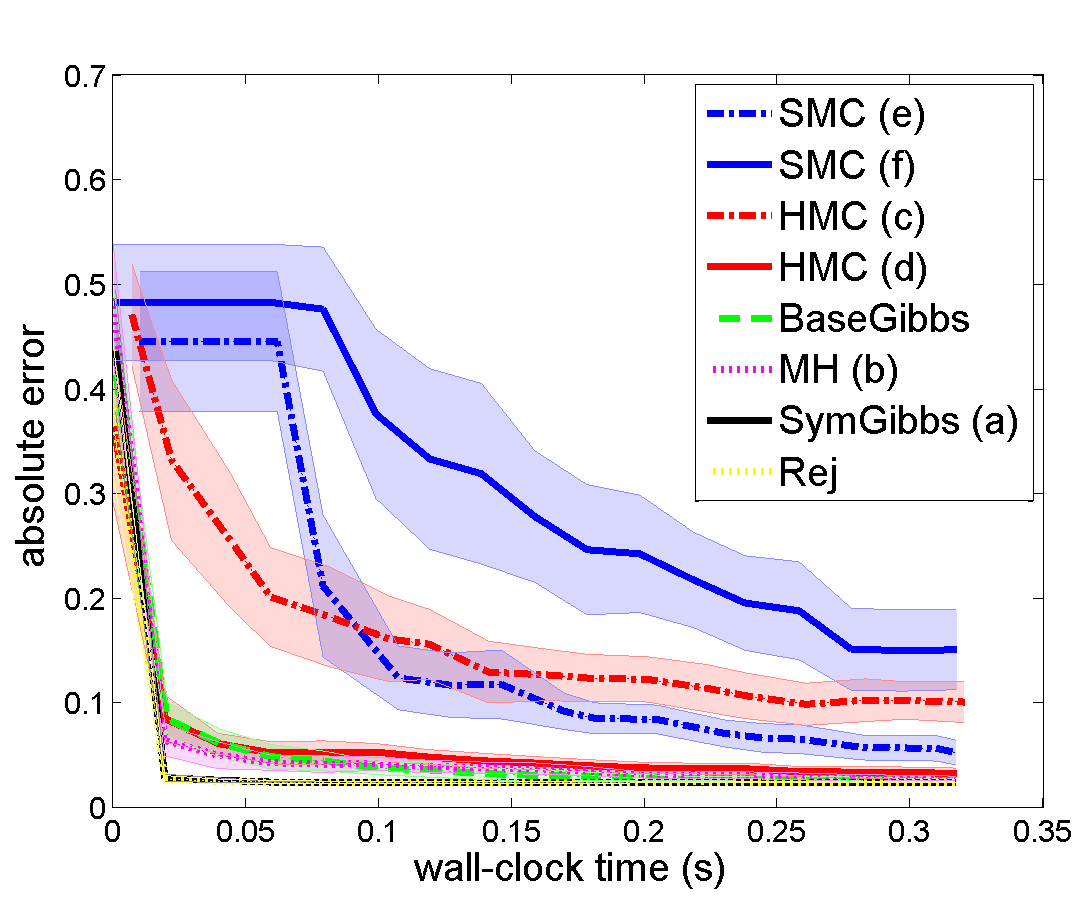
\includegraphics[width=0.8\linewidth, height=125pt]
{plotsx/vis-col/err-vs-time__param2-shaded.pdf}
%{Figs/plots/collision/err-vs-time__param4-shaded.pdf}
      \caption{
%Error as a function of wall clock time (s) for the (asymmetric) collision model using MCMCs with same configurations as in Figure~\ref{fig:mom2}. 
Absolute error vs time in the \emph{asymmetric collision model}. (Most algorithms correspond sub-figures of Fig.~\ref{fig:mom2}.)
 }
\label{fig:asymmetric}
\end{figure}





%Ex 2;  Fig 1
%%%%%%%%%%%%%%%%%%%%%%%%%%%%%%%%%%%%%%%%%%%%%%%%%%%%%%%%%%%%%%%%%%%%%%%%%%
\begin{figure*}[t!]
\vspace{-0mm}
\begin{center}
\begin{tabular}{ccc}
   \hspace{-5mm} 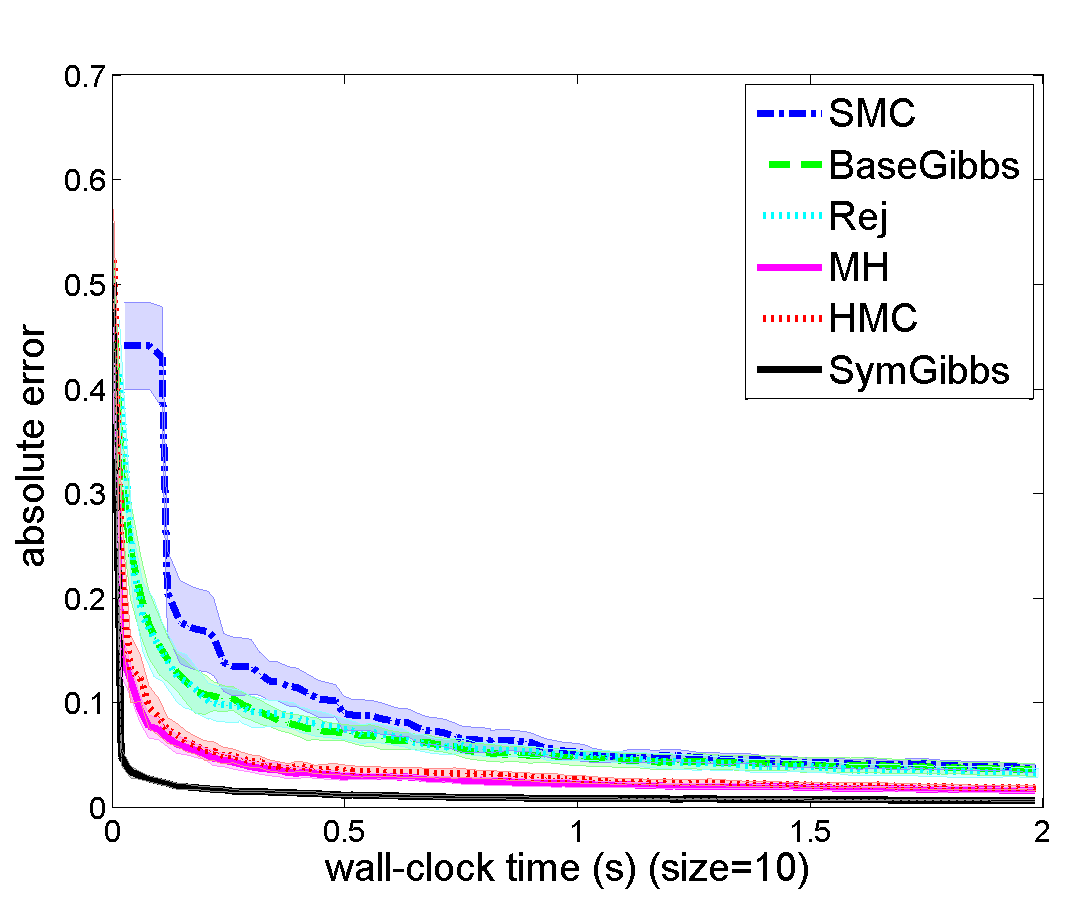
\includegraphics[width=\nnn\textwidth, height=\nnh\textwidth]{plotsx/collisionx/err-vs-time__param5-shaded.pdf} 
& \hspace{-3mm} 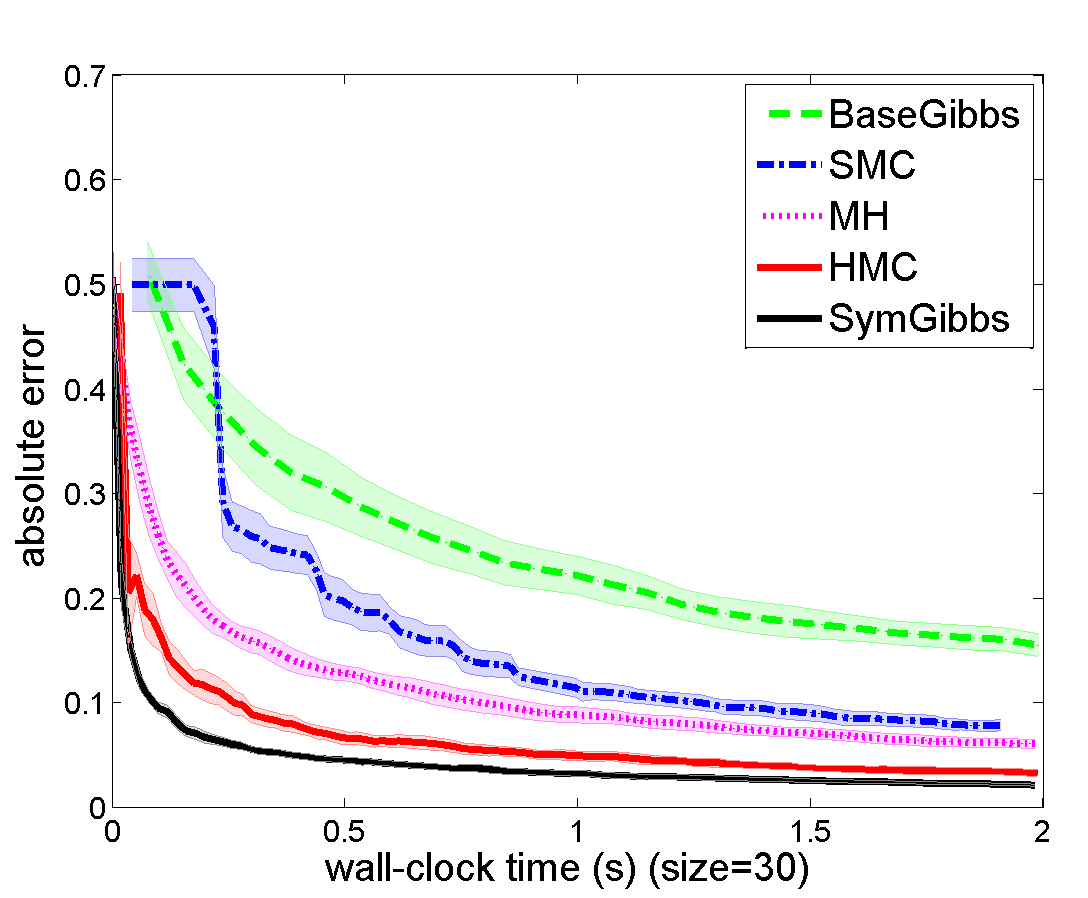
\includegraphics[width=\nnn\textwidth, height=\nnh\textwidth]{plotsx/collisionx/err-vs-time__param15-shaded.pdf} 
& \hspace{-3mm} 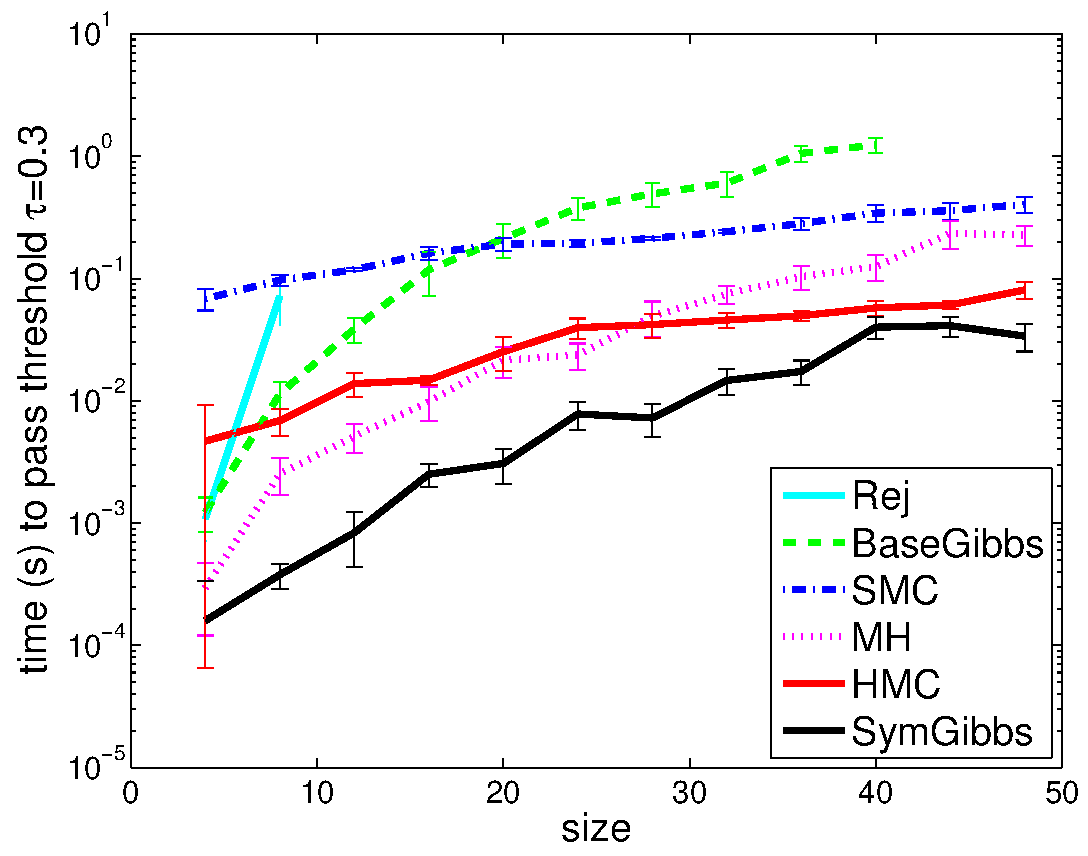
\includegraphics[width=\nnn\textwidth, height=\nnh\textwidth]{plotsx/collisionx/time_vs_param-errorbar.pdf}%collision/collisionTimeVsSize.png}
\vspace{-1.5mm}
\\
\hspace{-5mm} \footnotesize(a) 
& \hspace{-4mm} \footnotesize(b) 
& \hspace{-3mm} \footnotesize(c) \\
\multicolumn{3}{c}{}
\end{tabular}
\end{center}
\vspace{-8mm}
\caption{\footnotesize 
MCMC Convergence measurements in the symmetric multi-object collision model: 
Absolute error vs time for collision of (a) 4 and (b) 20 objects; (c) Time to reach error threshold $\tau=0.3$.}
\label{fig:multi-object.mom}
\vspace{-4mm}
\end{figure*}
%%%%%%%%%%%%%%%%%%%%%%%%%%%%%%%%%%%%%%%%%%%%%%%%%%%%%%%%%%%%%%%%%%%%%%%%%%


%Ex 2;  Fig 1
%%%%%%%%%%%%%%%%%%%%%%%%%%%%%%%%%%%%%%%%%%%%%%%%%%%%%%%%%%%%%%%%%%%%%%%%%%
\begin{figure*}[t!]
\vspace{-0mm}
\begin{center}
\begin{tabular}{ccc}
   \hspace{-5mm} 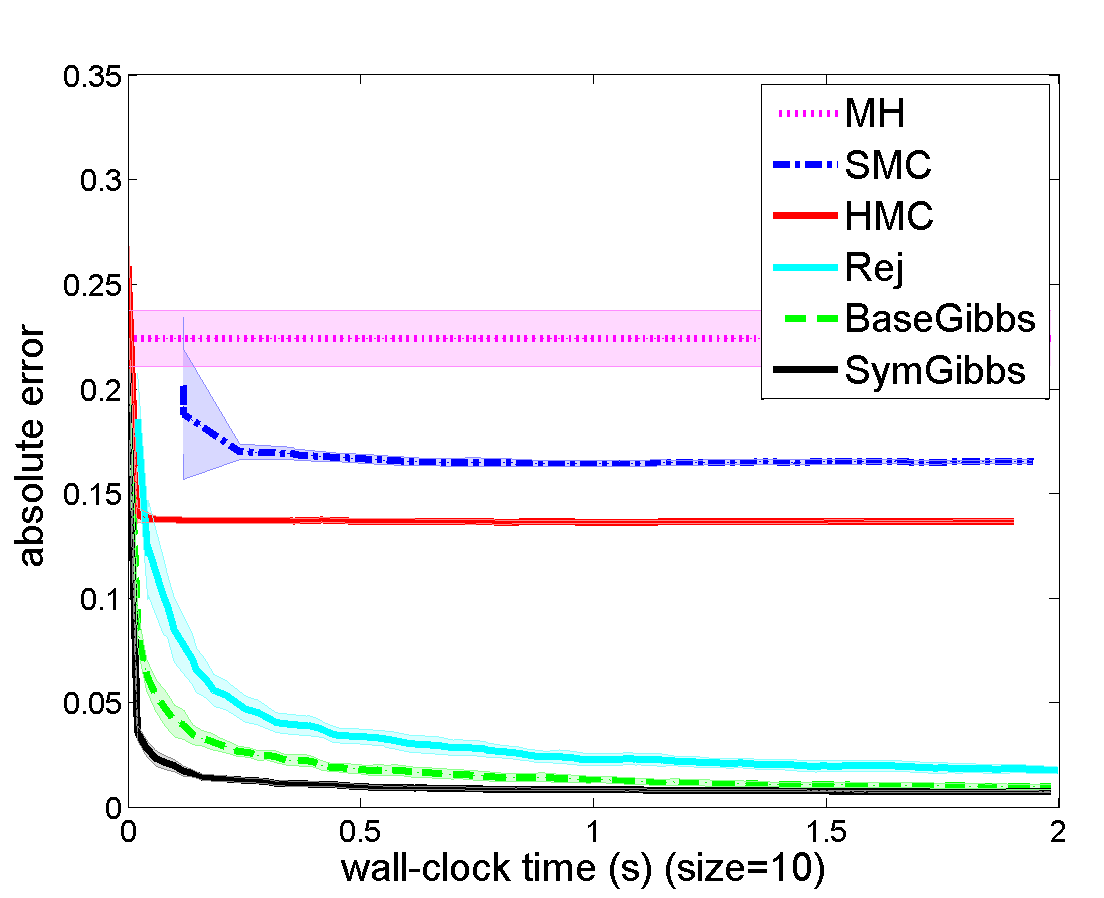
\includegraphics[width=\nnn\textwidth, height=\nnh\textwidth]{plotsx/conductancex/err-vs-time__param10-shaded.pdf} 
& \hspace{-3mm} 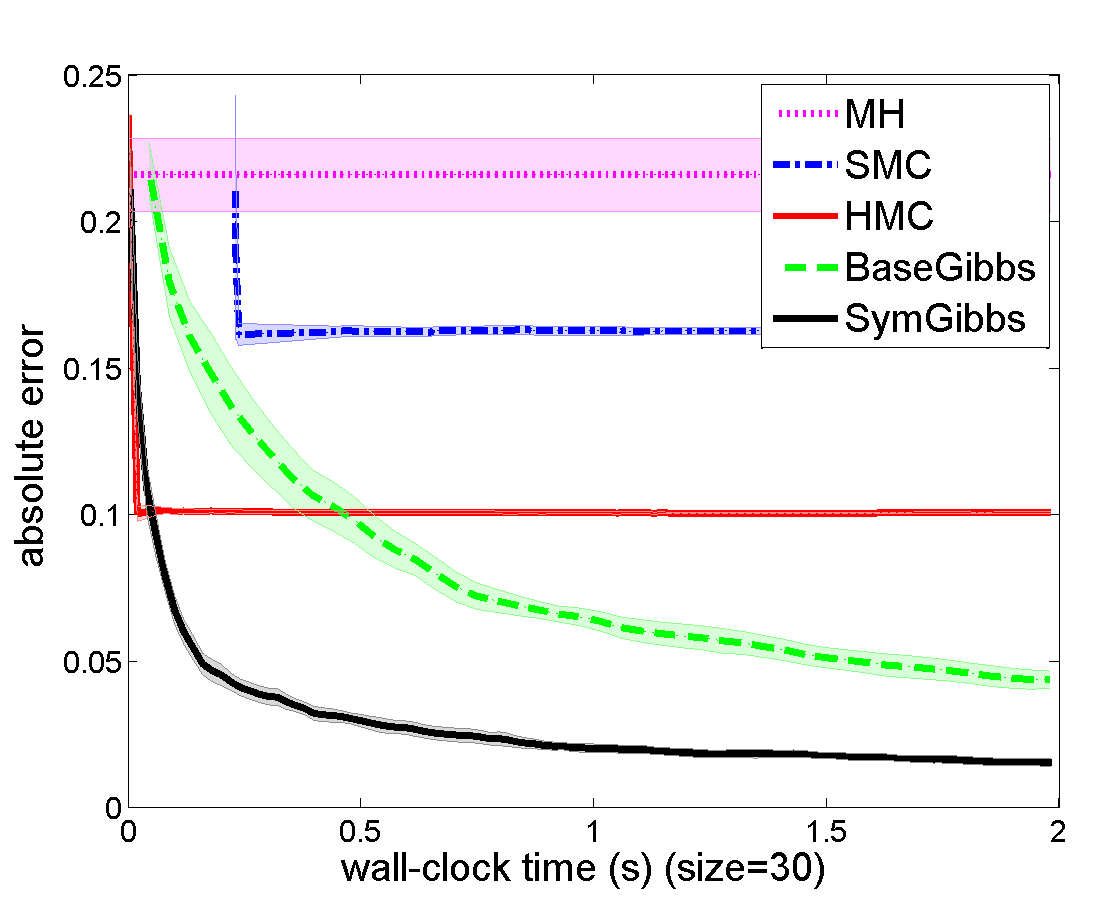
\includegraphics[width=\nnn\textwidth, height=\nnh\textwidth]{plotsx/conductancex/err-vs-time__param30-shaded.pdf} 
& \hspace{-3mm} 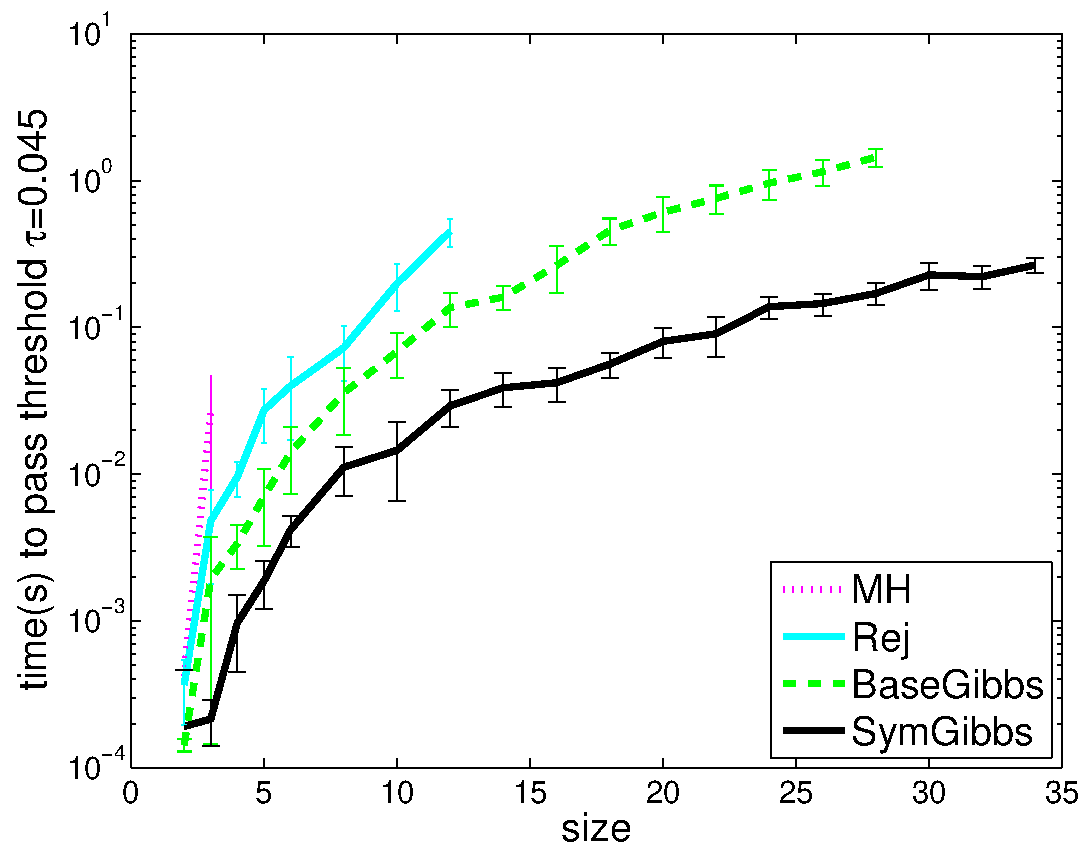
\includegraphics[width=\nnn\textwidth, height=\nnh\textwidth]{plotsx/conductancex/time_vs_param-errorbar.pdf}
\vspace{-1.5mm}
\\
\hspace{-5mm} \footnotesize(a) 
& \hspace{-4mm} \footnotesize(b) 
& \hspace{-3mm} \footnotesize(c) \\
\multicolumn{3}{c}{}
\end{tabular}
\end{center}
\vspace{-8mm}
\caption{\footnotesize 
MCMC Convergence measurements in the building wiring model: 
Absolute error vs time for a model with (a) size 4 (i.e.\ 4 paralleled resistors) and (b) size 30; (c) Time to reach error threshold $\tau=0.045$.}
\label{fig:resistor}
\vspace{-4mm}
\end{figure*}
%%%%%%%%%%%%%%%%%%%%%%%%%%%%%%%%%%%%%%%%%%%%%%%%%%%%%%%%%%%%%%%%%%%%%%%%%%




\subsubsection{Symmetric multi-object collision model} %In the second experiment,

%We study the role of model size on the performance of MCMC methods. We cannot rely on \emph{MCMC convergence diagnostics} methods \citep{cowles1996markov} because they can produce misleading results in case MCMCs do not converge to the ground truth, a scenario that as we will see, for highly complex posteriors is not improbable. Meanwhile, we cannot rely on rejection sampling to approximate the Ground truth since its performance on the studied model deteriorates drastically in dimension. Our solution is to conduct tests on symmetric models for which the posterior ground truth can be computed manually.

Consider a variation of the collision model in which $n$ objects collide.  
%by assuming that %collide. But we omit the sequential dependencies of velocities s.t.\ 
Let all $V_i$ and $M_i$ share a same uniform prior $U(0.2, 2.2)$ and the constraint be $\sum_{i=1}^n{M_i V_i} = P_{\text{tot}}$. 
The symmetry enables us to compute the posterior ground truth means  values  manually:
\begin{equation}\footnotesize
\label{e:col.GT}
M^* = V^* = \sqrt{P_{\text{tot}} / n} %\left(\frac{P}{n}\right)^{0.5}
\end{equation}
Conditioned on $P_{\text{tot}} = 1.5 n$, all masses $M_i$ and velocities  $V_i$ are queried. 
%The tested algorithms running on the reduced-dim posterior are: symbolic Gibbs (see Section~\ref{sect:symbolic.gibbs}), 
%baseline Gibbs (CDF computation per sample), 
%MH (Metropolis-Hastings tuned manually), 
%MH automatically tuned %to reach the acceptance rate of 0.234 
%after \citep{roberts1997weak})\footnote{\label{foot:tuning} Among 200 equidistant proposal variances in %interval $(0, 0.1]$ 
%the one is chosen for which the acceptance rate is closer to 0.24. } and rejection sampling. Among the samplers that add noise to determinism, Stan's Hamiltonian MCMC with noise (variance) parameter $\sigma_P = 0.05$ and Anglican's SMC with noise parameter $0.1$ are plotted. The noise parameters are chosen manually trying to maximize the convergence rate. Other parameters are Stan and Anglican's default setting.
%By (\ref{e:col.GT}), $a_k$, the average  of $k$-th sample vector $\bvec{s}^{(k)}$, is expected to be $\sqrt{1.5}$; therefore, as the overall sampling error measure, 
%$\mathbb{E}[|{\xi} - {\xi}^*|]$ 
%$\mathbb{E}[|\bvec{a} - \bvec{a}^*|]$ is computed where $\bvec{a}$ is the vector of $a_k$ (for $k$ ranges be the number of taken samples) and all entries of vector $\bvec{a}^*$ are 1.5.
By (\ref{e:col.GT}), all elements of the the expected query vector $\bvec{a}^*$ are $\sqrt{1.5}$.

%For each algorithm 15 Markov chains are run and at consecutive time slots, their corresponding point-to-point means and standard errors are computed. 
The absolute error vs time (depicted in figures~\ref{fig:multi-object.mom}.a \& b for 4 and 20 objects respectively)\footnote{
Note that the dimensionality of the random variable space is twice the number of objects because each object is associated with a mass and a velocity node. %Conditioned on the total momentum, reduced-dim space is 19D and algorithms that add noise to the observation, deal with  a 21D space.
} and the time to reach error threshold measurements indicate that (SymGibbs) sampler constantly and significantly performs the best.

%We repeated the experiment for different model sizes but for the sake of space restrictions, we do not depict each plot individually. Instead we provide a single plot that summarizes the overall behavior of each sampler w.r.t.\ the model size. We notice that after a particular threshold, the comparative performance of the samplers remains fixed. Therefore, in Figure ???, for each sampler the (wall-clock) time (s) to reach a sampling error threshold (average) equal to 0.3 is plotted vs the model size.\footnote{ If we pick the error threshold to be too low, many samplers would never reach it. If it is too high, samplers pass it prior to be comparatively stable. On collision model, the manual error threshold choice (around) 0.3 happens to provide a fair compromise between these two requirements.  }%end footnote

  
%In the latter high-dimensional space, the rejection sampling has not been able to generate a particle. MH algorithms convergence rate is very low while the baseline Gibbs still perform well and the symbolic Gibbs performance is at least an order of magnitude better. Finally, Figure~\ref{fig:err-threshold-vs-size-collision} depicts the time to reach a fixed error threshold $T=0.2$ versus number of colliding objects. \\
%



\subsubsection{Building wiring model} 
We perform the convergence tests on a model with a more complicated observed determinism: 
Consider an electrical circuit composed of $n$, $10\Omega\pm5\%$ paralleled resistor elements $R_i$
(with priors $\pr(R_i) = U(9.5, \, 10.5)$).
% with bell-shaped tolerance distributions (truncated quadratics, positive in the range $[8, 12]$). The posterior tolerance distribution is computed when 
The resistors are inaccessible i.e.\ the voltage drop and the current associated with them cannot be measured directly.
Given the source voltage $V$ and the total input current $I$, the posterior distribution of element resistances is required.
Here the deterministic constraint is:
%Here, the observation can be stated as the following deterministic constraint:
\begin{equation} \footnotesize 
\label{e:reduced.mass}
 \frac{1}{R_1} + \ldots + \frac{1}{R_n} = c
\end{equation}
where $c = \frac{I}{V}$.
Equations if the form (\ref{e:reduced.mass}) are generally referred to as \emph{reduced mass} relationships and 
have applications in in electrical, thermal, hydraulic and mechanical engineering domains.

Let the observation be $c = {3n}/{(2*10.5 + 9.5)}$.
Due to the symmetry of the problem, the posterior ground truth mean is known:
\begin{equation*}
R_i^* = \frac{n}{c} = 10.6667\qquad \text{ for } i = 1, \ldots, n
\end{equation*}
%Stan and Anglican observation noise divergences are 0.02 and 0.07 respectively. Other settings are as before.

The experimental results, as plotted in Figure~\ref{fig:resistor} illustrate that even 
in low dimensions (as in Figure~\ref{fig:resistor}-a) the algorithms that soften determinism by adding noise do not converge to the manually computed ground truth. This (and the results of the former experiments) indicate that approximation of determinism with noise may not be a good choice.

Figure~\ref{fig:resistor}-b shows that on higher dimensions, only variations of Gibbs sampling on the $\delta$-collapsed model converge to the ground truth.% (that we are certain about because of symmetry argument). 

%Figure~\ref{fig:resistor}-a \& \ref{fig:resistor}-b  illustrate sampling error vs time (s) for models with 4 and 30 resistors (respectively). In this model, even in low dimensions  It can be seen that only variations of Gibbs sampling on the reduced model converge to the ground truth (that we are certain about because of symmetry argument). 

Manual computations verify that in this model, 
conditioning on 
(\ref{e:reduced.mass}) leads to high degree terms in the posterior fraction.
This might be a reason for the poor performance of the MH-based algorithms:
There exists highly dense regions in the posterior that act as traps for MH based algorithms.

%Here and in the quantitative experiments that will follow, regardless to the parameter tuning, the performance of algorithms where determinism is softened by noise is much lower than the algorithms with $\delta$-collapsed models.
